\chapter{Data and methodology}\label{ch:3}

This chapter presents the experimental design used in this cross-sectional study (\sectref{sec:3.1}), the L2 learner as well as control groups who participated in the production experiment (\sectref{sec:3.2}), the experimental procedure (\sectref{sec:3.3}), and the methods employed to analyse and evaluate the data (\sectref{sec:3.4}).


\section{Experimental design}\label{sec:3.1}

\begin{sloppypar}
As already mentioned, the experimental design of the present study is related to the combination of different methods employed by the international project (\textit{Inter-)Fonología del Español Contemporáneo} ((I)FEC; see \citealt{PustkaEtAl2016,PustkaEtAl2018}), and which in turn is modelled on the French corpus project (\textit{Inter}{}-)\textit{Phonologie du Français Contemporain} ((I)PFC) \citep{RacineEtAl2012}.\footnote{The present study differs from the (I)FEC methodology in certain respects, in part because data collection for this study started before a definitive description of the methodology used in the (I)FEC project was published, but also because this study pursues slightly different objectives. Additionally, the present study also includes Italian, which precluded using the narrative text of (I)FEC, which is designed for Spanish.} Data for the present study and different follow-up studies in the area of L2 phonology were gathered by means of an hour-long production experiment divided into four different parts, which were presented to all participants (i.e., L2 learners as well as control groups) in the following order (as explained below, not all parts were considered for the final analysis of the present study):
\end{sloppypar}\largerpage[-2]

\begin{enumerate}[label={(\arabic*)}]
\item
A \textit{repetition} \textit{(imitation)} \textit{task}: Participants were asked to listen carefully to an audio playback of a series of 101 words, one word at a time, as uttered by three native speakers of (Peninsular) Spanish (or Italian), repeating each word before listening to the next. The words in the list were selected to exemplify various segmental phenomena and the position of the accented syllable.\pagebreak



\item Two \textit{reading} \textit{tasks}:


\begin{enumerate}[label={\alph*.}]
\item
  Participants were asked to read a Spanish or Italian translation of the chapter entitled “Drunkard” from \textit{The Little Prince} (French original \textit{Le Petit Prince}, Antoine de Saint-Exupéry, 1943). The chapter is short and easy to understand, and because it is largely framed as a conversation, it includes both declarative and interrogative sentences. This feature differentiates the present study from other studies, which tend to use mostly narrative texts (e.g., \textit{The North Wind and the Sun} or \textit{El sueño bastante animal} in \citealt{PustkaEtAl2016,PustkaEtAl2018}).


\item
  Participants were asked to read aloud a list of the same words as used in the repetition task. As already explained, these words were selected according to various segmental and suprasegmental phenomena, and additionally, according to the presence or absence of an orthographic accent (in the case of Spanish).
\end{enumerate}


\item
          A \textit{semi-directed} \textit{conversation} (see \citealt{Silva-CorvalánEnrique-Arias2017}, cf. \citealt{PustkaEtAl2018}): This task was intended to obtain spontaneous (L2) speech and thus gather information about the participants’ individual characteristics. Here participants informally answered a set of prepared questions about (1) themselves (place of residence, hobbies, family, travel experience), (2) their reasons for studying Spanish/Italian, (3) whether they regarded the target language as difficult for them individually or in general for Czech/German native speakers, (4) what kinds of difficulties (if any) they felt they had with Spanish/Italian pronunciation, and (5) what Spanish/Italian sounds and other features they considered different from Czech/German. The latter two questions were intended to elicit information on learners’ implicit/explicit phonological awareness with regard to their L2. The prepared questions from this conversation were carried out between the first two tasks and the final task because it was felt that doing so would ensure a relaxed atmosphere during recording. (Some questions of this task were left out in the case of the L1 native speakers.)



\item
          An intonation questionnaire called \textit{Discourse Completion Task} (DCT) (see below), in which participants were presented with a particular daily context and asked how they would react to it verbally in Spanish/Italian.
\end{enumerate}


In addition to the four main parts, L2 learners were recorded in their L1 (Czech and German), reading the story \textit{The Little Prince} and doing the DCT questionnaire that was developed for the present study.



The data from the fourth task constitutes the focus of the present study.\footnote{Results based on other parts of the experiment have already been presented. For example, \citet{PeškováEtAl2017} analysed the data from the word list (reading task) and found that the orthography of the reader’s native language significantly influenced the duration of stressed vowels in their L2 speech. Since the acute accent (´) signals a long vowel in Czech but lexical stress in Spanish, the L1 Czech learners tended to lengthen orthographically marked vowels in their L2 Spanish.} Though the DCT is a method originally developed for research in interlanguage pragmatics (\citealt{Blum-KulkaEtAl1989, KasperDahl1991, Félix-Brasdefer2010}), it has subsequently been adapted and applied in many intonation studies, starting with \citet{Prieto2001} on the intonation of Catalan. The DCT is an inductive (and partially interactive) method in which the researcher uses a kind of guided questionnaire to present the speaker with a series of everyday situations to which s/he is supposed to react spontaneously. For example, the participant is told the following situation: “You go into a shop you have never been in before and ask the shop assistant if they sell tangerines” and is expected to answer something like: “Hello, do you sell tangerines?” (from \citealt{PrietoRoseano2009-2013}). One such questionnaire in particular has successfully been used in recent intonation research across different L1 languages and their varieties (see, e.g., \citealt{PrietoRoseano2010} for ten different Spanish dialects; \citealt{FrotaPrieto2015} for nine Romance languages).



The original DCT for intonation of Romance languages (see, e.g., \citealt{PrietoRoseano2009-2013, FrotaPrieto2015}) was designed to be used with native speakers and was intended to elicit sample data of authentic L1 intonation contours for a wide variety of utterances. Hence, the questionnaire comprises descriptions of different situations, each one designed to prompt one of several different sentence types such as statements, yes/no questions, wh-questions, imperatives or vocatives with either pragmatically neutral or biased meanings (e.g., counter-expectational echo questions, confirmatory questions, statements of the obvious or command imperatives). This technique has proven to be very useful not only because it yields (semi\nobreakdash-)spontaneous, rather authentic data with a wide range of different melodic contours but also because its fairly standardized design facilitates comparisons across dialects and languages (\citealt[392]{FrotaPrieto2015}, for further advantages and shortcomings of the DCT method see \citealt{VanrellEtAl2018}).\largerpage[2]



Despite the fact that the intonation DCT was originally developed for L1 intonation research, I endeavour here to apply the method to L2 prosody too, taking into consideration several of the drawbacks noted above regarding the DCT method and adapting the method in accordance with the particular objectives and interests of this study:\footnote{Though the same prompt situations are described in all four versions of the questionnaire, given the differences between these four languages, it was impossible to control for segmental structure across them, since segmental or syllabic structure is likely to differ among these languages. But all this did not present an obstacle to applying the DCT to the present investigation.}\pagebreak



\begin{enumerate}[label={(\arabic*)}]
\item
          It comprised 25 situations for elicitation of different sentence types, which were limited to basic structures, namely declaratives, yes/no questions, wh-questions, imperatives and vocatives. Some examples are shown in \tabref{tab:3.1a} (see Appendix~\ref{app:a} for the full questionnaire).\footnote{The DCT was developed first for L2 Spanish and only later adapted for L2 Italian.}



\item
          In order to avoid difficulties in the task due to possible cultural differences or social factors, the instructions were simplified and the prompted contexts were common or stereotypical situations.



\item
          Each description of a context was accompanied by visual material (as in \citealt{GabrielEtAl2010}) embedded in a PowerPoint presentation. In other words, as participants listened to the description of the context, they were shown images depicting the situation on the screen.



\item\label{it:3:4}
          Target utterances were elicited in two steps:


\begin{itemize}\sloppy
\item First, the participant was asked to react to the situation spontaneously using his/her own words (consistent with the original DCT procedure).

\item Second, the participant was shown a prepared answer and asked to read it aloud, pronouncing it as naturally as possible in a way that was appropriate for the given context. These answers were based on the spontaneous verbal reactions produced in response to each context by native speakers.

\end{itemize}
\end{enumerate}

\begin{sidewaystable}
\small
\begin{tabularx}{\textwidth}{lQQQ>{\raggedright\arraybackslash}p{2cm}}

\lsptoprule

{No.} & {Situation prompt text, with intended response utterance in italics. Spanish version} & {Situation prompt text, with intended response utterance in italics. Italian version} & {English translation} & {Type of statement and formality of the context}\\
\midrule
01 & Te preguntan qué fruta prefieres. Dices que prefieres mandarinas. (¿Qué fruta prefieres?)

{\itshape -- Prefiero mandarinas.} & Ti chiedono che frutta preferisci. Tu rispondi che preferisci i mandarini.

{\itshape -- Preferisco i mandarini.} & They ask you what fruit you prefer. You say that you prefer tangerines. (What fruit do you prefer?)

\textit{-- I prefer tangerines}. & neutral

--

informal\\
\tablevspace
02 & Mira el dibujo y dime: ¿qué pasa aquí?

{\itshape -- Marisa come mandarinas.} & Guardate la foto e dimmi: che cosa sta succedendo?

\textit{--} \textit{Marisa mangia dei mandarini.} & Look at the picture and tell me what is happening here.

-- \textit{Marisa is eating tangerines.} & neutral

--

informal\\
\tablevspace
07 & Entras en una tienda donde nunca estuviste antes y preguntas si tienen mandarinas.

{\itshape -- ¿Tienen mandarinas?} & Entri in un negozio dove non siete mai stato prima e chiedi se hanno dei mandarini.

 \textit{-- Avete dei mandarini?} & You enter a store that you have never been in before and ask if they have any tangerines.

-- \textit{Have you got tangerines?} & neutral

--

formal\\
\tablevspace
08 & Acabas de comer con un amigo y ves que él se para delante de la pastelería. Pregúntale (todo asombrado porque acabaron de comer) si todavía tiene hambre.

{\itshape -- ¿Todavía tienes hambre?} & Proprio adesso hai pranzato molto con un amico e vedi che lui si ferma davanti alla pasticceria. Chiedi (molto sorpreso, perché avete finito il pranzo) se ancora ha fame.

\textit{--} \textit{Hai ancora fame?!} & You have just finished lunch with a friend and you see that he seems to have stopped in front of a pastry shop. Amazed -- since he just ate a big meal -- you ask him if he is still hungry.

-- \textit{You’re still hungry?!} & non-neutral

(echo)

--

informal\\
\midrule
\end{tabularx}
\caption{\label{tab:3.1a}Examples of situations used to elicit neutral statements and yes/no questions in L2 Italian and L2 Spanish.}
\end{sidewaystable}
\begin{sidewaystable}\ContinuedFloat
\small
\begin{tabularx}{\textwidth}{lQQQ>{\raggedright\arraybackslash}p{2cm}}

\midrule

{No.} & {Situation prompt text, with intended response utterance in italics. Spanish version} & {Situation prompt text, with intended response utterance in italics. Italian version} & {English translation} & {Type of statement and formality of the context}\\
\midrule
09 & Tus sobrinos hacen mucho ruido y no te dejan escuchar la televisión. Les preguntas si se quieren callar.

{\itshape -- ¿¡Quieren/queréis callarse?!} & I tuoi nipoti fanno un sacco di rumore e non ti lasciano guardare la TV. Gli chiedi se possono rimanere zitti.

\textit{--} \textit{Volete rimanere zitti?!} & Your nieces and nephews are making lots of noise and you can’t hear the television. You ask them to be quiet.

-- \textit{Will you be quiet?!} & non-neutral

(imperative)

--

informal\\
\tablevspace
10 & Pregúntale a tu amigo si quiere ir a tomar una cerveza contigo.

{\itshape -- ¿Vamos a tomar una cerveza?} & Chiedi al tuo amico se vuole andare a prendere una birra con te.

\textit{-- Andiamo a prendere una birra?} & Propose to a friend that the two of you go out for a beer.

-- \textit{Shall we go for a beer?} & neutral

--

informal\\
\tablevspace
11 & Estás en el autobús. Hay un asiento libre al lado de una señora mayor. Le preguntas si puedes sentarte.

-- \textit{Permiso, ¿me puedo sentar?} & Sali sul bus. C'è un posto libero accanto a una signora. Chiedi se puoi sederti.

-- \textit{Scusi, posso sedermi?} & You are on the bus and want to sit down next to an older woman. You ask her politely if the seat next to her is available and if you may sit down.

{\itshape -- Excuse me, may I sit down?} & neutral

--

formal\\
\tablevspace
21 & Te dicen que un amigo tuyo, Juan, se presenta para el puesto de presidente. No lo puedes creer y vuelves a preguntar.

{\itshape -- ¿Juan? ¿Presidente?} & Ti dicono che il tuo amico Giovanni si è presentato per la carica di presidente. Non ci puoi credere e chiedi di nuovo.

{\itshape -- Giovanni? Presidente?} & You hear that, John, a friend of yours, is running for president. You can’t believe it and ask again.

{\itshape -- John? For president?} & non-neutral

(emphatic)

--

informal\\
\lspbottomrule
\end{tabularx}

%\caption{\label{tab:3.1b}Examples of situations used to elicit neutral statements and yes/no questions in L2 Italian and L2 Spanish (continued).}
\end{sidewaystable}



The two-step method described in \ref{it:3:4} was based on a pilot study, where I observed that many L2 learners, especially those with a lower level of L2 proficiency, were reticent or less fluent when producing spontaneous utterances in the L2 but quite prepared to repeat what they knew to be an appropriate response if it was offered to them. Hence, the present study evaluated only the answers obtained in the second step. The advantage of this was that the utterances produced were identical across all tested L2 learners as well as control groups and thus easy to compare. The obvious drawback of this method is that the utterances produced thus were not semi-spontaneous, since they were read from a script. However, it is of interest to note that the reading of these utterances seemed more fluent and even more natural in comparison to participants’ first spontaneous productions, which were often hesitant and halting (this problem occurred even with some native speakers). It should also be mentioned that many spontaneous first answers were in fact very similar or identical to non-spontaneous read reactions and participant output exhibited no significant differences across the two tasks in terms of tonal contours (see \figref{fig:3.1}).




\begin{figure}
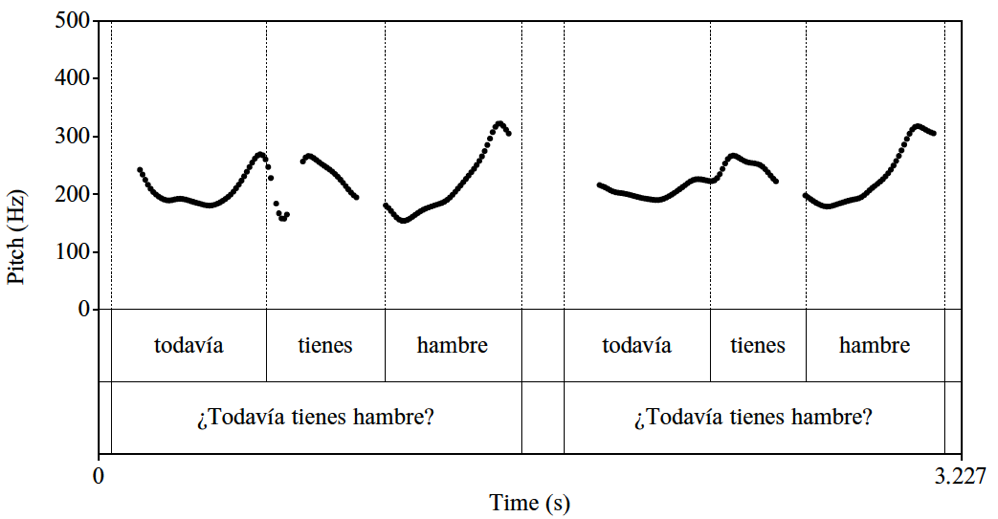
\includegraphics[width=\textwidth]{figures/a03HabilMethodology-img001.png}




\caption{Example of the elicited sentence \textit{¿Todavía tienes hambre?} (‘You’re still hungry?!’) as a semi-spontaneous answer (left) and as a read answer (right), produced by a German female learner of L2 Spanish (Ge\_09\_F).}
\label{fig:3.1}
\end{figure}



Interestingly, many speakers commented that, of the four parts of the experiment, the DCT was the most challenging, but at the same time the most interesting or entertaining task. Recall also that the DCT was recorded at the end of the whole experiment, by which point participants had forgotten that they were being recorded.


\section{Participants}\label{sec:3.2}

Participants were 60 adult L2 learners: 40 L2 Spanish learners (20 L1 Czechs and 20 L1 Germans), and 20 L2 Italian learners with L1 Czech. Besides their L1, the participants were also selected according to their “L2 proficiency level”. Half of them were independent (B) and another half proficient (C) users according to the \textit{Common European Framework of Reference for Languages} (CEFR). Furthermore, six native speakers of Spanish and six of Italian also took part as a control group. The participants received a small fee in compensation for their participation and all gave prior written consent to be recorded. Additionally, participants were asked whether they had been diagnosed with any hearing or speech disorder. There were no problems reported in this respect.



The Czech participants were recruited by the respective Faculties of Arts at Masaryk University in Brno and Charles University in Prague, the \textit{Hispánica} language school in Brno and the \textit{Instituto Cervantes} in Prague, institutions which kindly supported this project and facilitated the search for participants. It was not easy to find willing volunteers who fulfilled the same criteria, and in spite of all efforts the resulting set of participants was not completely balanced in terms of gender nor homogeneous in terms of L1 variety, the length of time spent living abroad and other variables summarized in Tables below. The recruitment and organisation of L1 German participants proved to be much easier, and this group was also more homogeneous than the Czech group. Nearly all of them were students at Osnabrück University, the two exceptions being two students at the University of Hamburg. All of them belonged to the same L1 -- Western North High German -- variety (cf. \sectref{sec:3.2.1}).



Aside from several of the L1 controls, none of the participants had any kind of close relationship with the interviewer. Moreover, they were unaware of the purpose of the study (i.e., L2 intonation), although they knew that the experiment dealt with research on second language speech. It should be noted that adjustments were made during the experimental procedure to accommodate par\-tic\-i\-pant-specific needs or output. For example, when a participant misunderstood a particular DCT situation, the context description was repeated, up to three times. However, when producing utterances, participants often corrected their output too. No participant displayed an insufficient L2 proficiency to warrant the exclusion of his/her data. By contrast, output from one male Czech L2 Spanish learner (Cz\_03) had to be excluded from the study because of his very high-proficiency (native-like) performance and his linguistic background, which was very different from that of the other participants; this derived from the fact that he had been teaching Spanish at a language school for over 10 years and had been married to a Colombian woman, and therefore was in constant contact with Spanish both at home and work.


\subsection{L2 Spanish learners (L1 Czech and L1 German)}\label{sec:3.2.1}\largerpage[2]

All forty L2 Spanish learners (20 L1 Czechs and 20 L1 Germans) were native speakers except for three Germans, who were (early) bilinguals with a Turkish, Russian or Portuguese background. Despite this fact, I included them in the analysis, for the following reasons.



\begin{enumerate}[label={(\arabic*)}]
\item
          They were born and grew up in Germany with L1 German being a dominant language in the sense used, for example, by \citet{Grosjean1982, Grosjean2008} and \citet{Montrul2013}.



\item
          Their L1 German was judged to be that of a German native speaker by ten other German native speakers in an ad hoc perception experiment.



\item
           Their L2 Spanish was judged to be “Spanish with a typical German accent” by five Spanish native speakers living in Germany in another perception experiment. In this perception experiment, the “foreign accent” of ten L2 Spanish learners with L1 German as well as seven L2 learners with other L1s (American English, Czech, Greek, Italian, Portuguese, Russian, Slovak) was rated independently by a set of Spanish native speakers.
\end{enumerate}\largerpage[2]


The tables below (\tabref{tab:3.2}--\ref{tab:3.3a} for Czech learners and \tabref{tab:3.4}--\ref{tab:3.5a} for German learners) give detailed information about the 40 L2 Spanish participants with regard to gender, age, occupation, L1 variety, Spanish proficiency, language experience abroad, age of L2 learning, language use (i.e., active use of Spanish per week at the time of the interview) and knowledge of other foreign languages.

As already noted, one half of the speakers in each group were independent L2 users (B1--B2) and the other half were proficient L2 users (C1--C2). The average age when the participants began to acquire Spanish was roughly the same for the two groups (CZ: 17 years old; GE: 18 years old). The two groups also shared the fact that English had been the L2 they acquired first, with exception of two Czech speakers (Cz\_02, Cz\_18) whose first L2s were German and Russian, respectively. The two areas with greatest differences between the groups were the frequency of active use of Spanish per week at the time of the experiment and the time spent in a Spanish-speaking country. Whereas Czech participants reported using Spanish actively almost eight hours a week on average, German participants did so only two hours a week. This was quite surprising, since all the German participants were students attending university and studying Spanish at the time of the experiment, whereas only ten Czech participants were studying Spanish at university. Concerning the variety of Spanish to which they were exposed, participants reported being exposed to non-native as well as native Spanish-speaking instructors coming from mainland Spain, the Canary Islands or Latin American countries. As already pointed out in \chapref{ch:2}, it would have been very difficult to control for this potentially intervening factor because it would have implied accepting only those participants who had been exposed to one particular Spanish dialect. However, the majority of participants had had more contact with Peninsular Spanish or were currently in contact with it. Finally, it should be noted that the two groups differed in terms of the distribution of occupations, but this was due to the manner of their recruitment, as described above.\pagebreak


\begin{table}[p]
\begin{tabularx}{\textwidth}{lllQQ}

\lsptoprule

{Person} & {Gender} & {Age} & {Occupation} & {L1 variety}

{Bohemian (B)}

{Moravian (M)\footnote{See Czech dialectal map in \figref{fig:3.3}}}\\
\midrule
Cz\_01 & M & 30 & independent & M (Brno; dialect II)\\
Cz\_02 & M & 40 & teacher (German) & M (Prostějov; dialect II)\\
Cz\_04 & F & 29 & artist & M (Vítkov; dialect II)\\
Cz\_05 & F & 29 & shop assistant & M (Brno; dialect II)\\
Cz\_06 & F & 23 & student (Spanish) & B (Prague; dialect Ib)\\
Cz\_07 & F & 21 & student (Spanish) & B (Prague surround.; dialect Ib)\\
Cz\_08 & F & 20 & student (Spanish) & B (Teplice; north-western part of B.)\\
Cz\_09 & F & 24 & nurse & B (Prague; dialect Ib)\\
Cz\_10 & F & 27 & student (translation and interpreting) & B (Prague; dialect Ib)\\
Cz\_11 & F & 19 & student (Spanish) & M (Třebíč; dialect II)\\
Cz\_12 & M & 33 & web designer & B (Prague; dialect Ib)\\
Cz\_13 & F & 31 & administrative assistant & B (Čáslav; dialect Ib)\\
Cz\_14 & M & 22 & student (Spanish) & B (Prague surround.; dialect Ib)\\
Cz\_15 & F & 24 & student (Spanish) & B (Prague surround.; dialect Ib)\\
Cz\_16 & F & 20 & student (Spanish) & B (Prague; dialect Ib)\\
Cz\_17 & M & 20 & student (Spanish) & B (Prague; dialect Ib)\\
Cz\_18 & F & 23 & student (Spanish) & B (Prague; dialect Ib)\\
Cz\_19 & M & 34 & shop assistant & B (Prague; dialect Ib)\\
Cz\_20 & F & 45 & secretary & B (Prague; dialect Ib)\\
Cz\_21 & M & 31 & manager & B (Prague; dialect Ib)\\
\lspbottomrule
\end{tabularx}
\caption{\label{tab:3.2}Gender, age, occupation and L1 variety of L2 Spanish participants (with L1 Czech).}
\end{table}

\begin{table}[p]
\small
\begin{tabularx}{\textwidth}{ll>{\raggedright\arraybackslash}p{.25\textwidth}QQQ}

\lsptoprule

{Person} & {Proficiency} & {Experience in a L2 area} & {Age at onset of acquisition} & {Active Spanish per week} {(hours)} & {Other} {L2s\footnote{The following abbreviations of L2 were used: ARAB (Arabic), CAT (Catalan), CRO (Croatian), DU (Dutch), EN (English), FIN (Finish), FR (French), GE (German), HU (Hungarian), ITA (Italian), LAT (Latin), POL (Polish), POR (Portuguese), RU (Russian), SPA (Spanish), SLO (Slovak), SWE (Swedish), TU (Turkish)}}\\
\midrule
Cz\_01 & C2 & 1 year in different locations in Spain, 1 year in different Latin American countries & 22 & 5 & EN, RU\\
\tablevspace
Cz\_02 & B1 & short visits to different locations in Spain & 35 & 1 & EN, GE, RU\\
\tablevspace
Cz\_04 & B2 & short visits to different locations in Spain & 20 & 2 & EN, GE\\
\tablevspace
Cz\_05 & B1 & short visit in Catalonia & 14 & 2 & EN, CRO\\
\tablevspace
Cz\_06 & C1 & short visits to different locations in Spain, Mexico, Guatemala & 17 & 20 & EN, GE\\
\tablevspace
Cz\_07 & B2 & no stay abroad & 16 & 1--2 & EN, POL\\
\tablevspace
Cz\_08 & B2 & no stay abroad & 15 & 20 & EN, CAT\\
\tablevspace
Cz\_09 & B2 & 1 year in different locations in Spain & 21 & 10 & EN, GE\\
\tablevspace
Cz\_10 & B2 & short visits to different locations in Spain, Mexico & 13 & 10 & EN, ITA, POR\\
\tablevspace
Cz\_11 & C1 & 1 month in the south of Spain & 17 & 8 & EN, FR, GE, POR, LAT, CAT\\
\midrule
\end{tabularx}
\caption{\label{tab:3.3a} Foreign language background of L2 Spanish participants (with L1 Czech).}
\end{table}

\begin{table}[p]\ContinuedFloat
\small
\begin{tabularx}{\textwidth}{ll>{\raggedright\arraybackslash}p{.25\textwidth}QQQ}

\midrule

{Person} & {Proficiency} & {Experience in a L2 area} & {Age at onset of acquisition} & {Active Spanish per week} {(hours)} & {Other} {L2s}\\
\midrule
Cz\_12 & B2 & short visits to different locations in Spain and Central America & 24 & 2 & EN, FR, GE\\
\tablevspace
Cz\_13 & C2 & 5 years in Spain & 16 & 3 & EN, GE, POR, RU\\
\tablevspace
Cz\_14 & C1 & short visits to different locations in Spain & 17 & 2–3 & EN, FR\\
\tablevspace
Cz\_15 & C1 & 6 months in Barcelona and short visits to different locations in Spain & 10 & 3 & EN, CAT\\
\tablevspace
Cz\_16 & C2 & short visits to different locations in Spain & 10 & 40\footnote{At the time of recording, the speaker was exposed to Spanish almost 40 hours a week because of her temporary job in an international company.} & EN\\
\tablevspace
Cz\_17 & C1 & 3 months in Valencia & 13 & 4 & EN\\
\tablevspace
Cz\_18 & C1 & 10 months in Valencia;

short visits to Cuba & 17 & 8 & EN, DU\\
\tablevspace
Cz\_19 & B2 & 1 month in northern Spain & 10 & 2 & EN, FR, ITA\\
\tablevspace
Cz\_20 & B1 & short visits to different locations in Spain & 19 & 1 & EN, FR, RU\\
\tablevspace
Cz\_21 & C1 & 2 years in Barcelona & 14 & 1 & EN\\
\lspbottomrule
\end{tabularx}

%\caption{\label{tab:3.3b} Foreign language background of L2 Spanish participants (with L1 Czech) (continued).}
\end{table}

\begin{table}[p]
\begin{tabularx}{\textwidth}{lllQ>{\raggedright\arraybackslash}p{3.2cm}}

\lsptoprule

{Person} & {Gender} & {Age} & {Occupation} & {L1 variety}

{(West Low German)}\\
\midrule
Ge\_01 & M & 37 & student, teacher (Spanish) & Ibbenbüren\\
Ge\_02 & F & 24 & student (Spanish) & Osnabrück\\
Ge\_03 & M & 26 & student (Spanish) & Osnabrück\\
Ge\_04 & F & 24 & student (Spanish) & Bünde\\
Ge\_05 & F & 20 & student (Spanish) & Lohne\\
Ge\_06 & F & 27 & student (Spanish) & Osnabrück\\
Ge\_07 & F & 28 & student (Spanish) & Hamburg\\
Ge\_08 & F & 27 & student (Spanish) & Hamburg\\
Ge\_09 & M & 21 & student (Spanish) & Osnabrück\\
Ge\_10 & M & 21 & student (Spanish) & Osnabrück\\
Ge\_11 & M & 24 & student (Spanish) & Osnabrück\\
Ge\_12 & F & 24 & student (Spanish) & Osnabrück\\
Ge\_13 & F & 21 & student (Spanish) & Osnabrück\\
Ge\_14 & M & 26 & student (Spanish) & Osnabrück\\
Ge\_15 & F & 23 & student (Spanish) & Osnabrück\\
Ge\_16 & F & 25 & student (Spanish) & Georgsmarienhütte\\
Ge\_17 & F & 22 & student (Spanish) & Osnabrück\\
Ge\_18 & F & 27 & student (Spanish) & Osnabrück\\
Ge\_19 & F & 23 & student (Spanish) & Osnabrück\\
Ge\_20 & F & 25 & student (Spanish) & Münster\\
\lspbottomrule
\end{tabularx}

\caption{\label{tab:3.4}Gender, age, occupation and L1 variety of L2 Spanish participants (with L1 German).}
\end{table}

\begin{table}[p]
\small
\begin{tabularx}{\textwidth}{ll>{\raggedright\arraybackslash}p{.25\textwidth}QQQ}

\lsptoprule

{Person} & {Proficiency} & {Experience in a L2 area} & {Age at onset of acquisition} & {Active}

{Spanish per week} & {Other}

{L2s}\\
\midrule
Ge\_01 & C1 & short visits to different locations in Spain & 32 & 3 & EN\\
\tablevspace
Ge\_02 & C1 & 6 months in Chile & 20 & 4 & EN, FR, ITA\\
\tablevspace
Ge\_03 & B2 & 5 months in Cádiz & 20 & 2 & EN, LAT\\
\tablevspace
Ge\_04 & C2 & 2 years in Lanzarote & 17 & 2 & EN, FR\\
\tablevspace
Ge\_05 & B2 & no stay abroad & 15 & 0.5 & EN, FR\\
\tablevspace
Ge\_06 & C1 & no stay abroad & 17 & 2 & EN, FR\\
\tablevspace
Ge\_07 & C1 & 6 months in Barcelona & 14 & 0 & EN, CAT, FIN, HU, ITA, SWE\\
\tablevspace
Ge\_08 & C1 & 6 months in Alicante & 17 & 0 & EN, FR, POR, RU\\
\tablevspace
Ge\_09 & B1 & short visits to different locations in Spain & 14 & 4 & EN, FR\\
\tablevspace
Ge\_10 & B2 & short visits to different locations in Spain & 13 & 2 & EN, FR\\
\tablevspace
Ge\_11 & B2 & 1 year in Mexico and different places in Spain & 15 & 3 & EN, FR\\
\midrule
\end{tabularx}

\caption{\label{tab:3.5a}Foreign language background of L2 Spanish participants (with L1 German).}
\end{table}

\begin{table}[p]\ContinuedFloat
\small
\begin{tabularx}{\textwidth}{ll>{\raggedright\arraybackslash}p{.25\textwidth}QQQ}

\midrule

{Person} & {Proficiency} & {Experience in a L2 area} & {Age at onset of acquisition} & {Active}

{Spanish per week} & {Other}

{L2s}\\
\midrule
Ge\_12 & C1 & 6 months in Cádiz & 20 & 2 & EN, FR\\
\tablevspace
Ge\_13 & B2 & short visits to different locations in Spain & 16 & 3 & EN, FR\\
\tablevspace
Ge\_14 & C1 & 5 months in Valladolid & 16 & 1 & EN

(2L1 = RU)\\
\tablevspace
Ge\_15 & B2 & 6 months in Costa Rica & 17 & 5 & EN, FR\\
\tablevspace
Ge\_16 & C2 & 9 months in Galicia,

many short visits to different Spanish-speaking countries & 19 & 2 & EN, FR

(2L1 = TU)\\
\tablevspace
Ge\_17 & B2 & 3 months in Andalucía & 16 & 2 & EN, LAT\\
\tablevspace
Ge\_18 & B1 & short visits to different locations in Spain & 23 & 2 & EN, LAT\\
\tablevspace
Ge\_19 & B2 & short visits to different locations in Spain & 21 & 3 & FR, DU, EN (2L1 = POR)\\
\tablevspace
Ge\_20 & C1 & 3 months in Madrid,

6 months in Alicante & 17 & 2 & EN, FR\\
\lspbottomrule
\end{tabularx}

%\caption{\label{tab:3.5b}Foreign language background of L2 Spanish participants (with L1 German) (continued).}
\end{table}\clearpage


With regard to their L1 variety, the German participants constituted a more homogenous group, since they all spoke one main German variety, namely, Western North High German (\figref{fig:3.2}).

\begin{figure}[p]
%%\includegraphics[width=\textwidth]{figures/a03HabilMethodology-img002.tif}
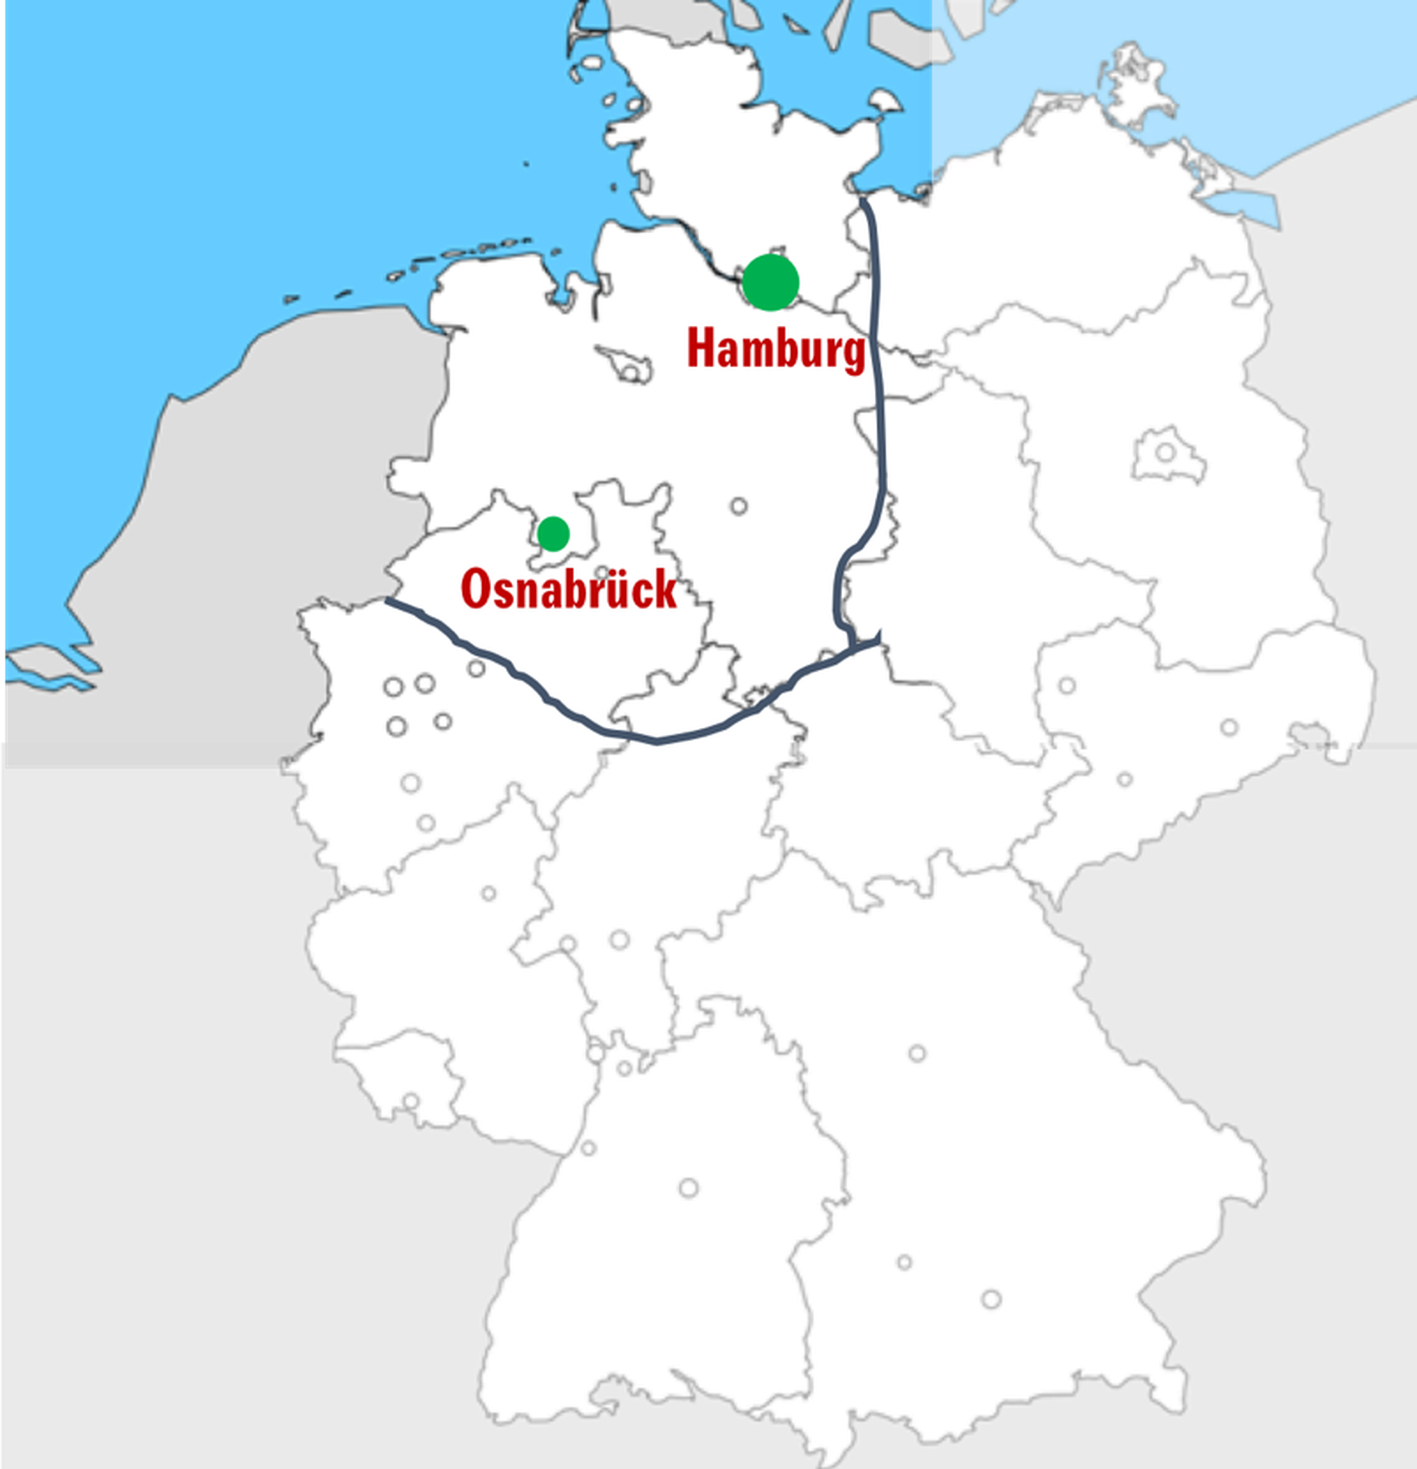
\includegraphics[width=.7\textwidth]{figures/a03HabilMethodology-img002-new.png}
\caption{The geographic distribution of Western North High German (own representation).}
\label{fig:3.2}
\end{figure}



In contrast, the Czech participants came from two main dialectal areas, Bohemian and Moravian (see, e.g., \citealt{Cvrček2010, ŠimáckováEtAl2012}), whose distribution is illustrated in \figref{fig:3.3}. These two dialects of Czech may -- according to the literature -- diverge slightly in intonation, as we noted in \chapref{ch:2} (see \chapref{ch:4}).




\begin{figure}[p]
%%\includegraphics[width=\textwidth]{figures/a03HabilMethodology-img003.tif}
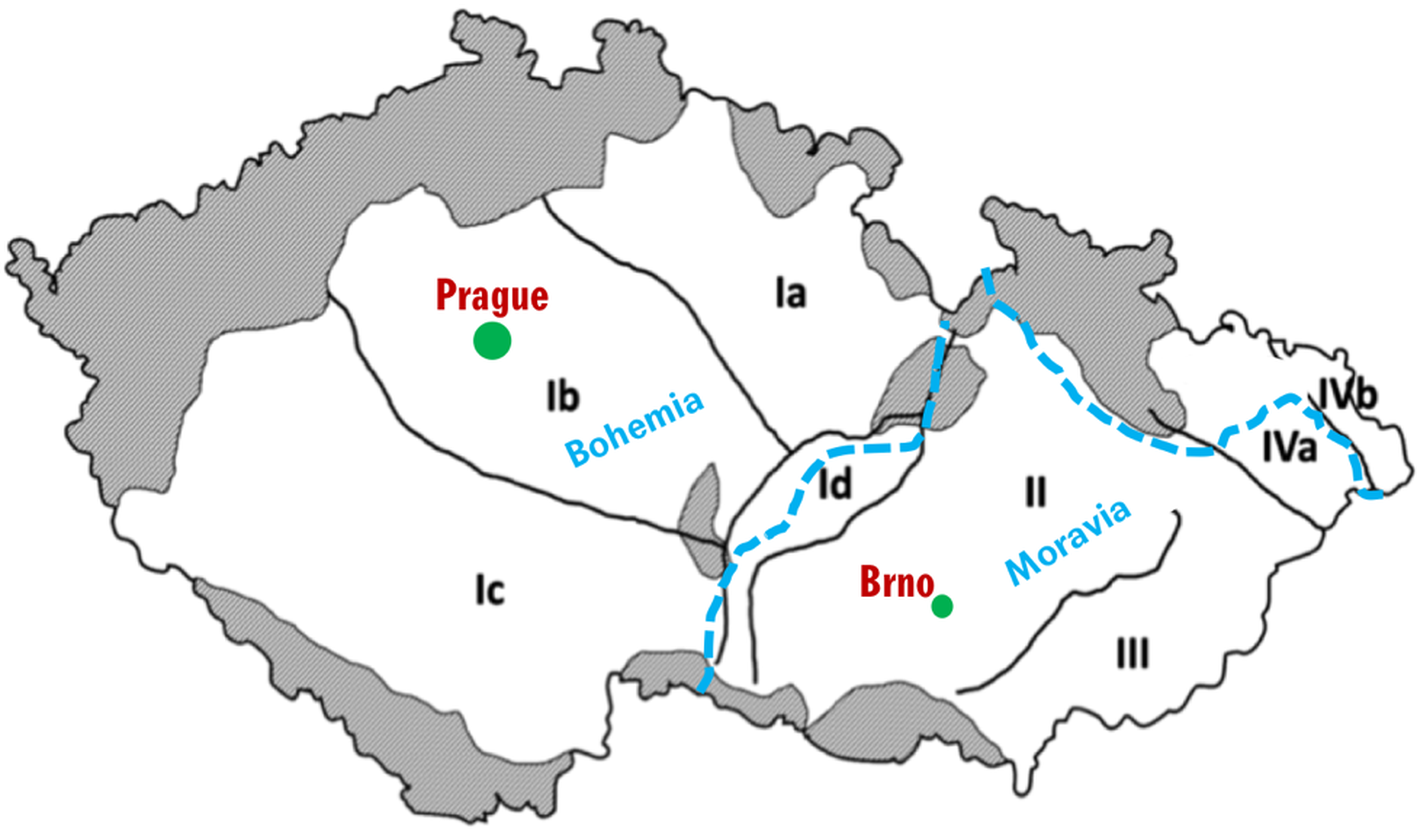
\includegraphics[width=.7\textwidth]{figures/a03HabilMethodology-img003-new.png}
\caption{Czech dialect map according to \citet{Kloferová2017}.\label{fig:3.3}}
\end{figure}



The fact that the Czech participants reflected two dialect groups was the consequence of practical considerations since, as noted above, I was dependent on cooperation with two universities as well as language schools for recruitment. The Bohemian participants came from Central Bohemia (Dialect Ib in \figref{fig:3.3}) and the Moravian speakers from the centre of the region (Dialect II), with the exception of three speakers who were from the region of Dialects Ia and Id. No speaker came from Silesia, the north-eastern part of the Czech Republic (Dialect IV). All this was considered in the results reported later.


\subsection{L2 Italian learners (L1 Czech)}\label{sec:3.2.2}

The recruitment of twenty L1 Czech learners of Italian (at B or C proficiency levels) was even more challenging than finding L2 Spanish speakers. This was due to not just the reasons outlined above but also the fact that Italian is less popular than Spanish as a foreign language in the Czech Republic at the moment. Thus, this group was especially heterogeneous in terms of L1 variety as seen in \tabref{tab:3.6}. Nor was the group at all balanced for gender, with males being grossly underrepresented.


\begin{table}[p]
\small
\begin{tabularx}{\textwidth}{lllQQ}

\lsptoprule

{Person} & {Gender} & {Age} & {Occupation} & {L1 variety}

{Bohemian (B)}

{Moravian (M)}

{Silesian (S)}\\
\midrule
Cz\_31 & F & 24 & student (Italian) & M (Starý Jičín; dialect III)\\
Cz\_32 & F & 38 & linguist & M (Veselí nad Moravou; dialect III)\\
Cz\_33 & F & 26 & student (Italian) & M (Břeclav; dialect III)\\
Cz\_34 & F & 23 & student (Italian) & M (Veselí nad Moravou; dialect III)\\
Cz\_35 & F & 23 & student (Italian) & S (Frýdek-Místek; dialect IVa)\\
Cz\_36 & F & 29 & student (Art history) & B (Hradec Králové; dialect Ia)\\
Cz\_37 & F & 30 & student (Italian) & M (Brno; dialect II)\\
Cz\_38 & F & 37 & travel consultant & M (Brno; dialect II)\\
Cz\_39 & F & 36 & PhD student (Italian literature) & M (Kuřim; dialect II)\\
Cz\_40 & F & 23 & student (Italian) & B (Pelhřimov; dialect Ic)\\
Cz\_41 & F & 26 & student (Italian) & S (Ostrava; dialect IVa)\\
Cz\_42 & F & 22 & student (Italian) & S (Ostrava; dialect IVa)\\
Cz\_43 & F & 24 & student (Italian) & M (Brno; dialect II)\\
Cz\_44 & M & 43 & information technology & B/M (Karlovy Vary, but more than 25 years living in Brno)\\
Cz\_45 & F & 22 & student (Italian) & M (Brno; dialect II)\\
Cz\_46 & M & 28 & student (Italian and general linguistics) & M (Brno; dialect II)\\
Cz\_47 & F & 24 & administration & M (Brno; dialect II)\\
Cz\_48 & F & 26 & student (andragogy) & B (Nové Město nad Metují; dialect Ia)\\
Cz\_49 & F & 27 & administration in international company (IT) & M (Brno; dialect II)\\
Cz\_50 & F & 31 & recruitments (personal agency) & M (Strážnice; dialect III)\\
\lspbottomrule
\end{tabularx}

\caption{\label{tab:3.6}Gender, age, occupation and L1 variety of L2 Italian participants (with L1 Czech).}
\end{table}


The participants also differed largely with regard to time spent living in an L2 area, active exposure to Italian per week and knowledge of other foreign languages (\tabref{tab:3.7a}).


\begin{table}[p]
\small
\begin{tabularx}{\textwidth}{ll>{\raggedright\arraybackslash}p{.25\textwidth}QQQ}

\lsptoprule

{Person} & {Proficiency} & {Experience in a L2 area} & {Age at onset of acquisition} & {Active Italian}

{per week} & {Other}

{L2s}\\
\midrule
Cz\_31 & C1 & 1 month in the Dolomites, 5 months in Siena & 18 & 2 & EN, FR\\
\tablevspace
Cz\_32 & B1 & short trips to different locations in Italy & 20 & 1 & EN, GE, SPA, FR\\
\tablevspace
Cz\_33 & C1 & 5 months in Padua & 19 & 4 & EN, FR\\
\tablevspace
Cz\_34 & B2 & short trips to different locations in Italy & 14 & 2 & EN, FR\\
\tablevspace
Cz\_35 & C1 & 16 months (Roma, Ravenna, Cervia) & 18 & 28 & EN, SPA\\
\tablevspace
Cz\_36 & B2 & three months in Parma, several weeks in Turin and Milan & 20 & 0 & EN, GE\\
\tablevspace
Cz\_37 & C2 & 3 months in Perugia; regular trips for work & 23 & 40 (work) & EN, FR\\
\tablevspace
Cz\_38 & C2 & 5 years in Toscana, Rome & 18 & 0 & EN, GE\\
\tablevspace
Cz\_39 & C2 & 6 years in San Benedetto del Tronto & 19 & 2 & EN, FR, SPA\\
\tablevspace
Cz\_40 & B2 & different short trips to Italy & 18 & 4 & EN, GE, FR\\
\midrule
\end{tabularx}
\caption{\label{tab:3.7a}Foreign language background of L2 Italian participants (with L1 Czech).}
\end{table}

\begin{table}[p]\ContinuedFloat
\small
\begin{tabularx}{\textwidth}{ll>{\raggedright\arraybackslash}p{.25\textwidth}QQQ}

\midrule

{Person} & {Proficiency} & {Experience in a L2 area} & {Age at onset of acquisition} & {Active Italian}

{per week} & {Other}

{L2s}\\
\midrule
Cz\_41 & C1 & 6 months in Rome; many short trips to Ravenna, & 19 & 5 & EN, GE\\
\tablevspace
Cz\_42 & B1 & 2 months in Genoa & 19 & 10 & EN, FR\\
\tablevspace
Cz\_43 & B2 & different short trips to different locations in Italy & 18 & 6 & EN\\
\tablevspace
Cz\_44 & B1 & 2 weeks in Calabria & 33 & 2 & EN, GE, SPA, FR, RU\\
\tablevspace
Cz\_45 & C1 & 4 months in Perugia & 20 & 4 & EN\\
\tablevspace
Cz\_46 & C1 & different short trips to different locations in Italy & 20 & 5-6 & EN, PORT\\
\tablevspace
Cz\_47 & B1 & 5 months in Verona & 20 & 0 & EN\\
\tablevspace
Cz\_48 & B2 & 14 months in Firenze & 11 & 2 & EN, FRA, ARAB\\
\tablevspace
Cz\_49 & C1 & different short trips to different locations in Italy & 12 & daily (Italian boyfriend from Abruzzo & EN, SPA, GE\\
\tablevspace
Cz\_50 & B1 & 3 months in Calabria & 25 & 1 & EN\\
\lspbottomrule
\end{tabularx}

%\caption{\label{tab:3.7b}Foreign language background of L2 Italian participants (with L1 Czech) (continued).}
\end{table}

\subsection{Control groups}\label{sec:3.2.3}

Since the intonation of different Spanish and Italian dialects has already been amply explored in the literature (see, e.g., \citealt{PrietoRoseano2010, GiliFivelaEtAl2015}), only six L1 (European) Spanish native speakers and six L1 Italian native speakers (Northern varieties) carried out the full experiment, the idea being that the data I obtained from these two control groups would serve as a basis for comparison with the experimental L2 learners’ groups and the literature (\tabref{tab:3.8} and \ref{tab:3.9}).


\begin{table}[p]
\begin{tabularx}{\textwidth}{lllQQ}
\lsptoprule
{Person} & {Gender} & {Age} & {Occupation} & {Dialect}\\
\midrule
Sp\_01 & F & 25 & student (Spanish and English) & Central-Southern Castilian\\
Sp\_02 & F & 24 & student (Spanish and German) & Central-Southern Castilian\\
Sp\_03 & F & 30 & university lecturer and researcher & Northern Castilian\\
Sp\_04 & F & 25 & university researcher & Northern Castilian\\
Sp\_05 & F & 38 & Spanish teacher & Central-Southern Castilian\\
Sp\_06 & F & 19 & student (secondary grammar school) & Central-Southern Castilian\\
\lspbottomrule
\end{tabularx}

\caption{\label{tab:3.8}L1 Spanish control group for the study (dialects based on \citealt{Hualde2005}).}
\end{table}

\begin{table}[p]
\begin{tabularx}{\textwidth}{lllQl}
\lsptoprule
{Person} & {Gender} & {Age} & {Occupation} & {Dialect}\\
\midrule
Ita\_01 & M & 20 & student (Italian) & Toscana\\
Ita\_02 & F & 29 & phonetician & Piemonte\\
Ita\_03 & F & 30 & university lecturer and researcher & Veneto\\
Ita\_04 & F & 21 & student (psychology) & Lombardia\\
Ita\_05 & F & 29 & German teacher & Piemonte\\
Ita\_06 & M & 30 & IT & Piemonte\\
\lspbottomrule
\end{tabularx}

\caption{\label{tab:3.9}L1 Italian control group for the study.}
\end{table}\clearpage


A second set of control data was obtained by having the experimental groups -- the Spanish and Italian L2 learners -- perform two of the experimental tasks (reading the chapter from \textit{The Little Prince} and doing the DCT) in their respective native languages. For the purposes of the present study, DCT data from twelve randomly selected L1 Czech and ten L1 German speakers were examined.


\section{Experimental procedure}\label{sec:3.3}

Czech participants carried out the experiment in March and May 2016, March 2017, February 2018 and February 2019 at either the Laboratory of Behavioural and Linguistic Studies \textit{LABELS} at Charles University in Prague, at the \textit{Hispánica} language school in Brno or in a soundproof laboratory at the Masaryk University Faculty of Informatics in Brno. Most of the German participants performed the experiment during the 2016 and 2017 summer and winter semesters at Osnabrück University; for two participants the experiment was run in May 2016 at the University of Hamburg.



In all cases, the experiments were carried out in a quiet location and the data were recorded directly as WAV files by means of a Marantz HD Recorder (PMD 671) and a Sennheiser microphone (ME 64) positioned at a distance of approximately 30\,cm from the speaker’s mouth (sample rate 44,100\,Hz, 16 bit). Subsequent data transcription along with acoustic analysis of all target utterances was performed with version 6.0.26 of the Praat software (\citealt{BoersmaWeenink1992-2019}). The whole experiment was recorded in an open, friendly and rather informal atmosphere in order to minimize tension on the part of participants and to ensure that recorded data were as natural as possible. The experimental materials and all instructions were presented to participants in the form of a PowerPoint presentation, so that direct intervention by the interviewer was limited. The whole experiment was conducted in the target language (Spanish or Italian); we switched into German or Czech only at the end of the experiment, when L1 data were collected. One recording session took around one hour and it was preceded by a general questionnaire soliciting demographic information and contact details of participants and a linguistic background questionnaire collecting information on factors such as age of L2 learning, amount of L2 experience, L2 use per week that can shape the participants’ individual characteristics of pronunciation (cf., \citealt{PiskeEtAl2001}).


\section{Analysis and measurements}\label{sec:3.4}

Although the full study involved the collection of data by means of a production experiment with several tasks, for the purpose of the present study only the data from the last experimental task, the DCT, will be analysed and discussed. While the DCT comprised a total of 25 prompt situations, only 18 situations per L2 learner have been selected for the final analysis offered here (see \chapref{ch:4}, \textit{\nameref{ch:4}}). The resulting corpus subjected to analysis thus consisted of a total of 1080 target items, including broad focus statements, pragmatically marked statements, different types of yes/no questions and wh-questions as well as vocatives. The intonation of imperatives and greetings was left aside for future investigation; exclamatives are treated in \citet{Pešková2022b}. The process yielded a total of 4.717 tonal events for final analysis and interpretation. This number comprises prenuclear pitch accents and nuclear accents with boundary tones. Each audio file was subjected to acoustic analysis by means of Praat software (\citealt{BoersmaWeenink1992-2019}), and orthographic transcription of the audio data as well as ToBI annotation of pitch contours (\sectref{sec:3.4.1}) were added. In order to capture further fine-grained phonetic differences between the learner varieties, F0 change as well as durational cues were measured (\sectref{sec:3.4.2}).


\subsection{Transcription of intonation}\label{sec:3.4.1}\largerpage

As already explained in \chapref{ch:2}, the transcription of F0 is based on two important tonal entities in Spanish and Italian, namely pitch accents (tones associated with tonic syllables) and boundary tones (tones associated with the edges of phrases). To date, the labelling of intonational data has generally been performed manually. Since manual labelling has been criticized for subjectivity and low reliability, I also employed a practical and innovative software tool for automatic transcription of (Spanish) intonation, called \textit{Etiquetador ToBI}, Eti\_ToBI \citep{Elvira-GarcíaEtAl2016}. Most importantly, the Eti\_ToBI transcriber performs a pitch track analysis based on linguistic features, using the Sp-ToBI system implemented in the script. Although the tool is intended to be applied to L1 Spanish data, in fact it works fairly well for Italian data and L2 data too (albeit requiring manual corrections).\footnote{As explained in \chapref{ch:2}, in Italian, there are two pitch accents and two boundary tones, hence four different labels, that are not assumed for Spanish: H*+L, L*+>H, and H!H\%, L!H\% respectively.} This automatic transcriber, running as a Praat script and transcribing up to 50 (simple) sentences per minute, labels all pitch accents and boundary tones. I will briefly explain how the tool works.



Before using Eti\_ToBI, a TextGrid with one interval tier (\textit{Text}) and one point tier (\textit{Break indices}) was created. The first tier, located underneath the spectrogram, obtained a phonetic transcription of the utterance analysed, divided into syllables (stressed syllables have to bear the IPA stress mark in order for Eti\_ToBI to be able to recognize the target tonal event).\footnote{The positions of the syllable boundaries as well as the end of IP-final words in Praat were determined according to several phonetic criteria -- such as formant structure, intensity and pitch periods -- which have been applied in previous studies on rhythm (see, e.g., \citealt{WhiteMattys2007, GrabeLow2002, GabrielKireva2014b}).}



In the second tier, levels of prosodic phrasing were annotated with break indices (BI). The Eti\_ToBI tool differentiates between three of these levels of structuring within the prosodic hierarchy: prosodic words (BI 1), intermediate phrases (ip) (BI 3) and intonational phrases (IP) (BI 4). An example of Eti\_ToBI tonal notation as applied to the Spanish sentence \textit{Se vende la casa bonita} ‘The nice house is for sale’ is given in \REF{ex:3:1}:


\ea\label{ex:3:1} \glllll {\textit{Se}]} {\textit{\textbf{ven}.de}]} {\textit{la}]}    {\textit{\textbf{ca}.sa}]} {\textit{bo.\textbf{ni}.ta}]}.\\
     {\hphantom{Se}\textbar}            {\hphantom{ven.de}\textbar}            {\hphantom{la}\textbar}               {\hphantom{ca.sa}\textbar}                   {\hphantom{bo.ni.ta}\textbar}\\
   {\hphantom{Se}BI 0}         {\hphantom{ven.de}BI 1}        {\hphantom{la}BI 0}           {\hphantom{ca.sa}BI 1}      {\hphantom{bo.ni.ta}BI 4}\\
          {}   (*)    {}   (*)            {(*)  (\%)}\\
\textsc{refl}   sell-\textsc{3ps.sg}    the\textsc{{}-f}     house         nice\textsc{{}-f}\\


\glt ‘The nice house is for sale.’
\z

After all TextGrids with the two corresponding tiers had been prepared, the script was run. As it applies the script, Eti\_ToBI offers the user the possibility of manually correcting the labels it proposes. On the present occasion this feature was particularly useful: First, the program was operating on L2 data, which show different F0 patterns. Second, the script is very sensitive to voiceless consonants (especially fricatives) and distorted some measurements. And finally, certain curve properties and interesting F0 shapes in the L2 data might have been missed had we relied solely on the points predetermined by the tool.


An example of the final output of the script is shown in \figref{fig:3.4}. The usual Praat output (spectrogram, F0 contour and orthographic transcription) is followed by a tier showing BI level numbers and three further tiers providing tonal information.




\begin{figure}
%%\includegraphics[width=\textwidth]{figures/a03HabilMethodology-img004.tif}
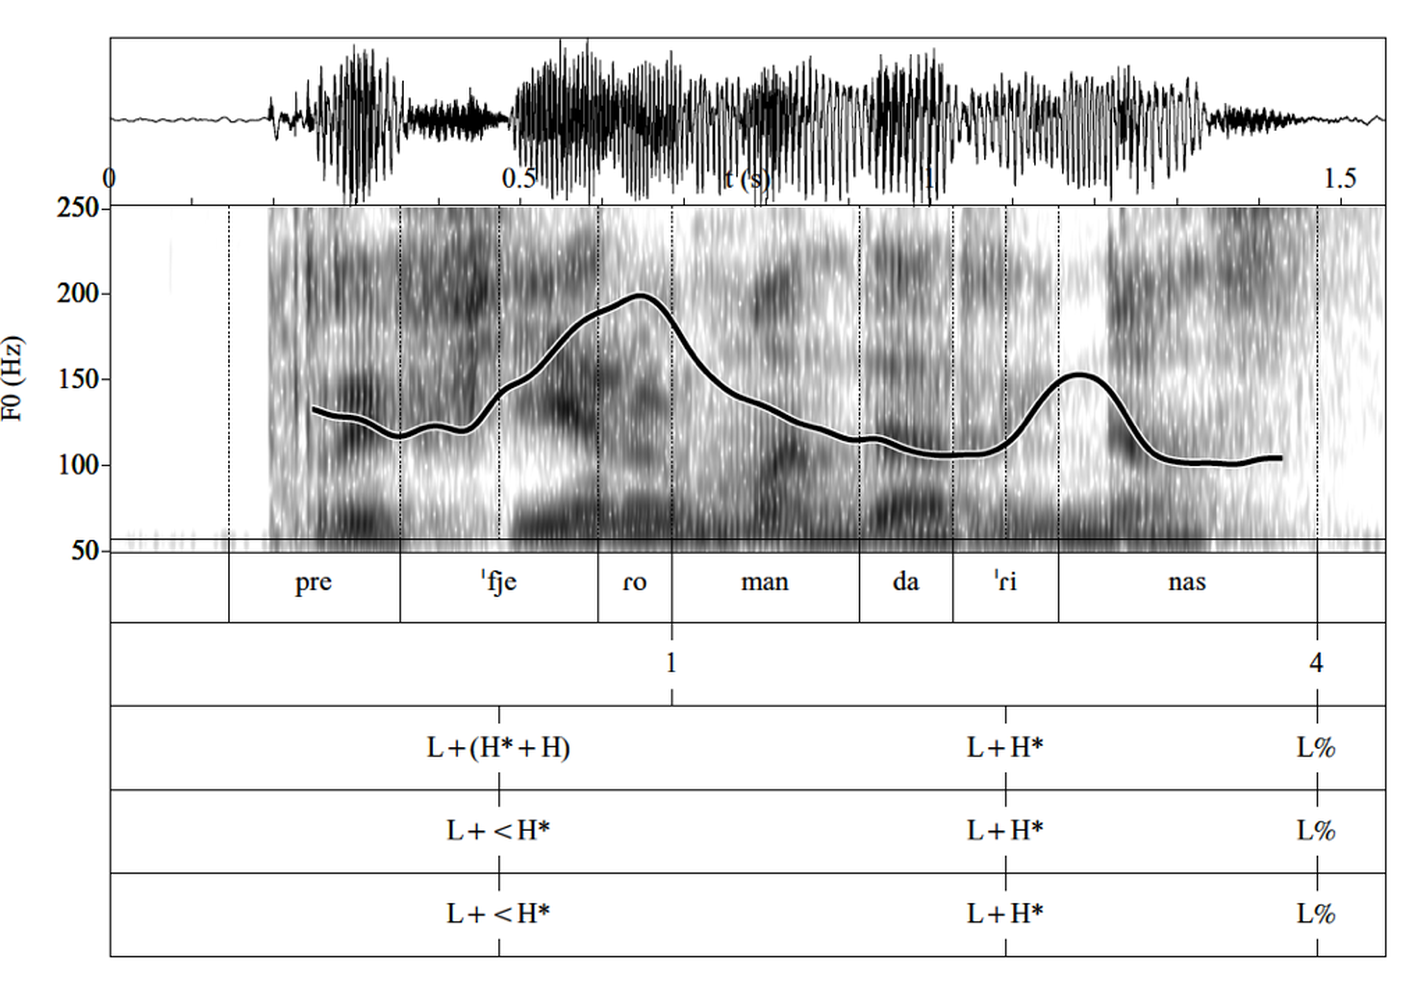
\includegraphics[width=\textwidth]{figures/a03HabilMethodology-img004-new.png}



\caption{Eti\_ToBI output for the L2 Spanish utterance \textit{Prefiero mandarinas} ‘I prefer tangerines’, produced by an L1 German participant (Ge\_03\_M).}
\label{fig:3.4}
\end{figure}



The first of these three tonal tiers comprises the \textit{surface} analysis of the utterance and allows tritonal accents (not included in the current ToBI systems).\footnote{In ToBI notation, all phonetically tritonal pitch accents are transformed into phonologically bitonal pitch accents, except for Argentinean “Italianized” Spanish, where the phonological inventory includes a tritonal L+H*+L accent \citep{GabrielEtAl2010}. Since Eti\_ToBI is designed to recognise intonational patterns of the ten dialects of Spanish described in \citet{PrietoRoseano2010}, initially the script offers the user the possibility of choosing whether the tritonal accent of Argentinean Spanish should be reported in one of the phonological tiers or not. This was very useful for the L1 and L2 Italian data.} The transcription of the prenuclear accent is thus a L+H*+H rise in the stressed syllable, which continues to rise in the post-stressed syllable. The smaller F0 movement of this complex tone is indicated between parentheses (in this case, L+(H*+H)). The authors of the Eti\_ToBI tool call this type of transcription a “transliteration of F0” (\citealt[775]{Elvira-GarcíaEtAl2016}) which contains many non-contrastive details similar to what is seen in a narrow phonetic transcription. Here, the Eti\_ToBI tags pitch movements greater than 1.5 semitones and takes into account three parameters: F0 shape, F0 alignment and F0 range. It thus gives detailed information about tonal events. In contrast to the Sp-ToBI conventions, which contain in total 14 labels for all tonal events (seven for pitch accents and seven for boundary tones), the surface transcription in Eti\_ToBI distinguishes between 13 labels for prenuclear pitch accents, 15 for nuclear pitch accents and 10 for boundary tones. Eti\_ToBI thus predicts a total of 150 possible nuclear configurations (all theoretically possible combinations of nuclear tones and boundary tones). The standardized (Spanish) ToBI permits only 61 combinations, though presumably not all combinations are available in the language.\footnote{As already noted in \chapref{ch:2}, the present study assumes a total of nine pitch accents and seven boundary tones. Although the proposed labels lack certain phonetic details, they appeared appropriate in the cross-linguistic comparison undertaken here and suitable for assessing results.}



The second tonal tier offers a \textit{deep} analysis (to use \citegen{Elvira-GarcíaEtAl2016} term), that is, a broad phonetic transcription, in which all tritonal pitch accents are converted into bitonal labels. This transcription was crucial for the present study. And finally, the third tonal tier provides a \textit{standardized} (conventionalized) transcription that “translates” some of the nuclear configurations into the current phonology-based (Spanish) ToBI. In fact, there are only a few small differences between the \textit{deep} and \textit{standardized} levels. For example, the configuration L+<H* H\% is converted into L+H* H\%, because L+<H* does not appear in the nuclear position in Spanish. Hypothetically, if we transform these three levels into the Spanish segmental level, the \textit{surface level} would give us complete information about non-contrastive sounds, the \textit{deep} \textit{level} would present a broad phonetic transcription containing only allophones important for one phonological system, and the \textit{standardized} \textit{level} would provide us with a phonological transcription, as illustrated in \REF{ex:3:2}.


\ea\label{ex:3:2}  Type of transcription

\gllll {\normalfont Orthographic transcription}      {\normalfont<vendido> ‘sold’}\\
{Narrow phonetic transcription}    [bɛ̃n̪ˈdi\textsuperscript{ð}o]\\
{Broad phonetic transcription}      [bɛnˈdiðo]\\
{Phonemic (phonological) transcription}   /benˈdido/\\
\z



What the transcription in \REF{ex:3:2} does not offer is information about formants (resonating frequencies of the vocal tract) F1 and F2, which are important for the acoustic characterization of all vowels (and which can be measured by means of speech software). By the same token, the ToBI transcription does not provide any detailed information on pitch range in F0 values (for example, a pitch accent realized with a rising tone L+H* does not say much about “how far” the L tone is from the H tone); nor does it provide further prosodic information such as the length of the event in ms. Some of these parameters will be measured and reported here separately (see \sectref{sec:3.4.2}).



Given all these considerations, the question arose as to how useful and reliable Eti\_ToBI would be for the purposes of the present study. I therefore ran a pilot experiment in which the program analysed and labelled 690 tonal entities (prenuclear pitch accents and nuclear configurations), and simultaneously I labelled the same materials manually. Though Eti\_ToBI proved unable to measure all instances (due to fricatives or creaky voices), in general agreement between the manual labelling and the Eti\_ToBI output was relatively high at 79\% (\textit{N} = 561). As noted by \citet[6]{Elvira-García2016}, “using Eti\_ToBI not only can speed up phonetician works in order to let them focus more in theory, but it can also highlight fails in the theoretical framework they use.” In other words, the script can correct or point out an erroneous interpretation, since it calculates differences in semitones. Nevertheless, we cannot forget that it is still a program, a bit hypersensitive to acoustic signal (mainly micro-prosody effects, voiceless consonants, fricatives and creaky voices), and the Praat pitch detection algorithm may thus perform inadequately (which can result in a distorted picture of the F0 contour and an erroneous label). Another issue to keep in mind is the effectiveness of Eti\_ToBI when it is run on L2 data. Although the program takes into account three levels of labelling, namely ToBI-standardized labelling (language-specific) and broad and narrow labelling (non-language-specific), it does not recognise the various phenomena that may result from L1 intonation interference. Hence, as noted above, manual correction of the automatic labelling proved to be unavoidable here. Since the present study deals with L2 data, transparent, consistent and especially non-language-specific labels were used for the analysis, which were already presented in Chapter 2. No inter-transcriber reliability of the labelling system of the present study has been assessed so far, but since the pilot study on labelling uniformity with Eti\_ToBI was run and the agreement was relatively high, the proposed labels can be deemed appropriate for the purposes of the study.



In spite of the transparent labels (presented in \chapref{ch:2}), transcription of L2 intonation was not straightforward in all cases and several difficulties were encountered in applying ToBI labels to the data. For example, when a pitch accent displayed a pitch movement that was only slightly rising, it was not clear whether to treat it as a L+H or just a H or L pattern. This was especially the case of “Czech” Spanish, which is characterized by a more flat pitch tracking. Following the Eti\_ToBI annotation parameters, the rising label LH was only assumed when the difference between L and H was larger than 1.5 semitones. Stress displacement represented another problematic issue for labelling, especially in data from several Czech participants (recall that Czech has initial stress). This is illustrated in \figref{fig:3.5}, where a Czech participant starts the sentence \textit{Prefiero mandarinas} from quite a high initial point (labelled as \textit{Hi}) and produces the overall pitch contour without any observable larger pitch movements. Interestingly, as a native Czech speaker myself I perceived Czech accenting on the first syllable, but Spanish native speakers consulted did perceive Spanish accenting (thus on the second syllable) here, perhaps because of additional non-tonal cues such as intensity or because of the access to the meaning. The target pitch accents associated with the stressed syllables (-\textit{fie-}, -\textit{ri-}) showed no slope at all or just a very slight one.




\begin{figure}[p]
%%\includegraphics[width=\textwidth]{figures/a03HabilMethodology-img005.tif}
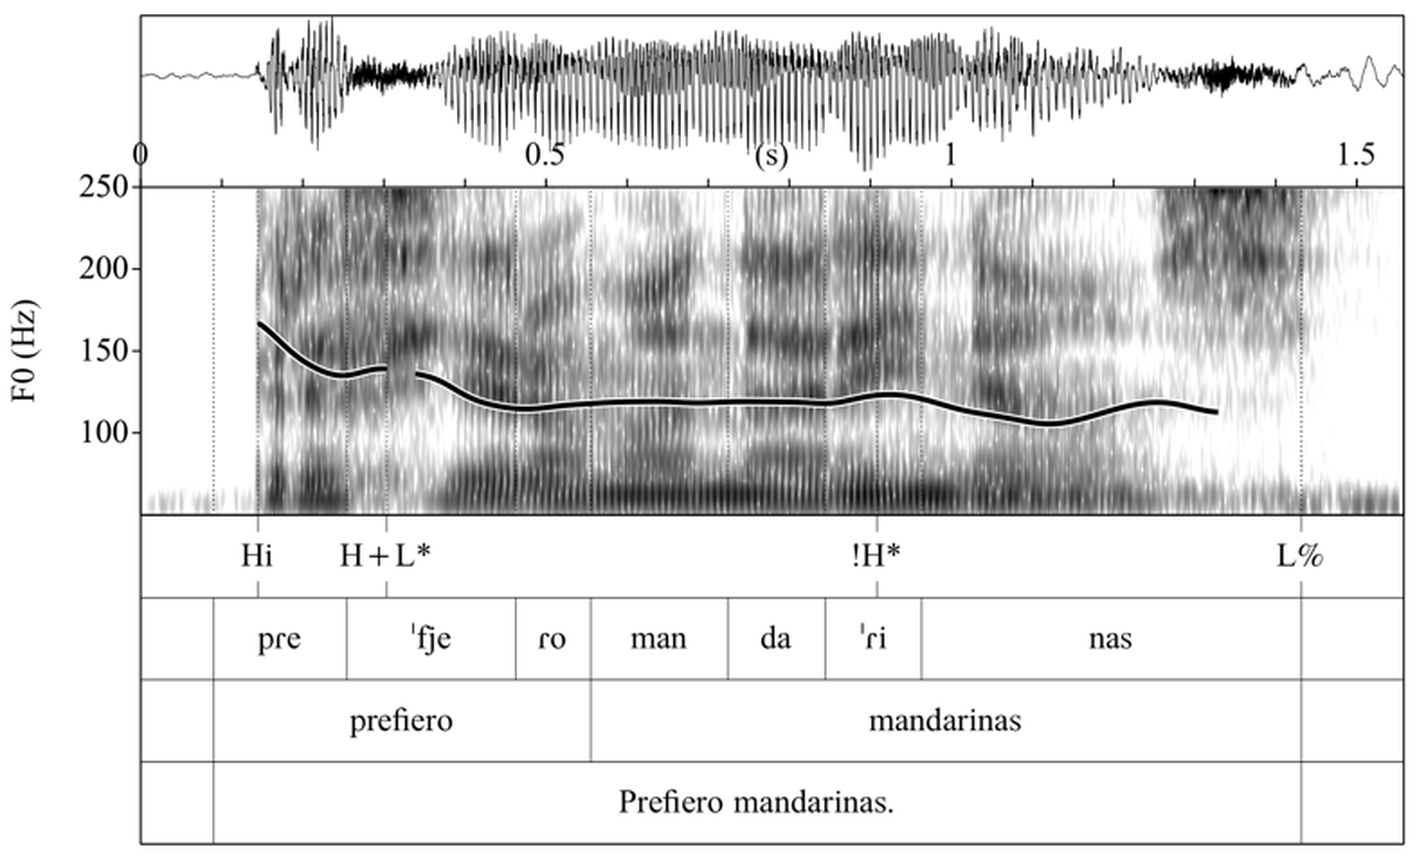
\includegraphics[width=.9\textwidth]{figures/a03HabilMethodology-img005-new.png}
\caption{Spectrogram and F0 trace for the statement \textit{Prefiero mandarinas} ‘I prefer tangerines’, produced by a L1 Czech learner of Spanish (Cz\_02\_M). It is realized with an initial high tone (Hi), a H+L* prenuclear pitch accent and a !H* L\% nuclear configuration.}
\label{fig:3.5}
\end{figure}

\begin{figure}[p]
%%\includegraphics[width=\textwidth]{figures/a03HabilMethodology-img006.tif}
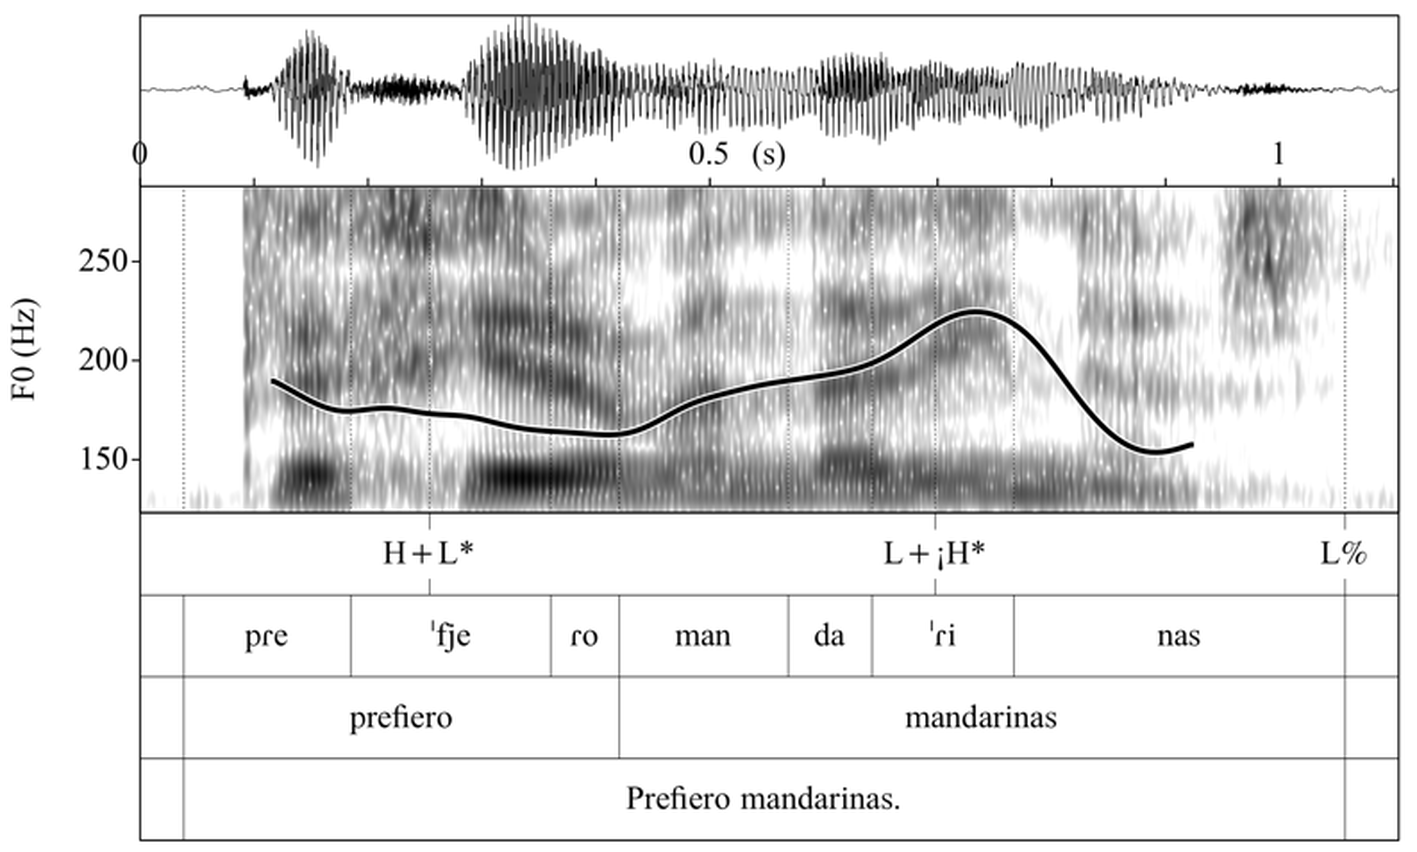
\includegraphics[width=.9\textwidth]{figures/a03HabilMethodology-img006-new.png}
\caption{Spectrogram and F0 trace for the statement \textit{Prefiero mandarinas} ‘I prefer tangerines’, produced by a Spanish native speaker (Sp\_01\_F). It is realized with a H+L* prenuclear pitch accent and a L+¡H* L\% nuclear configuration.}
\label{fig:3.6}
\end{figure}



The dilemma presented by such data was whether to mark the word on the first syllable \textit{pre-} with H* or on the second syllable -\textit{fie-} as H+L* and to decide which syllable anchored a pitch accent. In general, I opted for the second option (“Spanish” stress placement) because of similar scenarios observed in L1 Spanish native speakers too (\figref{fig:3.6}). In \figref{fig:3.6} the sentence-initial prenuclear position does not show the expected L+<H* rising pattern described in the literature. One possible interpretation of the falling prenuclear pattern (H+L*) with the peak on the first syllable may be that it either indicates deaccenting of the known material or represents a result of secondary stress.\footnote{A secondary stress in Spanish is an optional phenomenon and mostly observed in different forms of public or emphatic speech (\citealt{Hualde2007,Hualde2009, Hualde2010}).} Or it can be simply a case of variation of tonal patterns that is very similar to the variation one measures, for instance, in vowels that very often display a large dispersion and variability.


In some cases, a rising pattern occurs on a syllable other than the “target” syllable and the stress shift was not only visible but also clearly perceived. This is illustrated in \figref{fig:3.7}, where an L1 German learner of Spanish inappropriately places stress on the initial syllable of \textit{todavía} ‘still’ *[ˈto.ða.βi.a] instead of on the penultimate syllable [to.ða.ˈβi.a]. Other instances will be reported individually in \chapref{ch:4}.




\begin{figure}
%%\includegraphics[width=\textwidth]{figures/a03HabilMethodology-img007.tif}
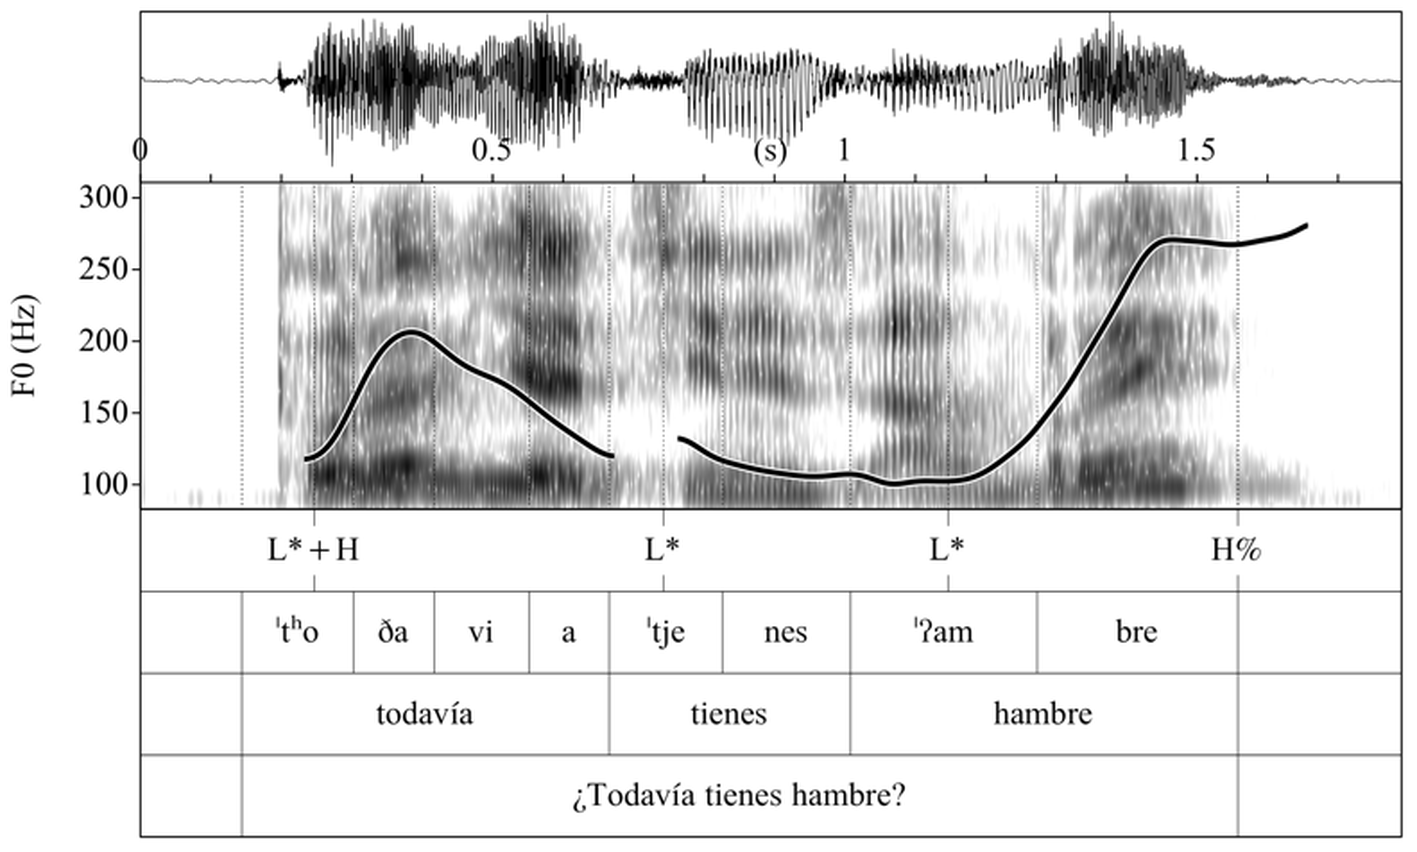
\includegraphics[width=\textwidth]{figures/a03HabilMethodology-img007-new.png}



\caption{Spectrogram and F0 trace for the yes/no question \textit{¿Todavía tienes hambre?} ‘Are you still hungry!?’, produced by an L1 German learner of Spanish (Ge\_03\_M).}
\label{fig:3.7}
\end{figure}


It should also be added that the tonal analysis of the L2 data (i.e., the application of ToBI labelling) was conducted in two directions and a total of four steps: (1) one sentence type per all speakers, (2) all sentences per one speaker, (3) step 2 was repeated after one month and, finally, (4) step 2 was repeated after six months again. Only about 4\% of all tonal events were modified again in the final labelling session.



Finally, besides the tonal annotation of pitch contours, the present study includes two additional parameters that are not integrated into the ToBI systems but which serve to capture further fine-grained phonetic differences between the learner varieties and the Spanish and Italian control groups. These parameters include (1) the pitch change for each tonal event, and (2) the duration of the whole sentences (measurements of duration cues concerning words and syllables will be left for future).


\subsection{Pitch change of tonal events and duration cues}\label{sec:3.4.2}

\begin{sloppypar}
Regarding the measurements of the pitch change, I marked the lowest and highest F0 points of every tonal event using the Praat command “Move cursor to minimum/maximum pitch”. As a rule, only voiced segments were measured and all F0 points were checked and corrected manually or removed from the results, if necessary. Not all F0 contours produced by speakers were ideal for pitch measurements due to devoicing, the presence of voiceless consonants or creaky voice. In those instances where the F0 was reduced due to creaky voice, the value obtained by the script was doubled \citep{ArvanitiEtAl2017} or repaired by the Praat MAUSMOOTH script (“MAnually and AUtomatically SMOOTHed”; \citealt{Cangemi2015}), which permits the user to make manual corrections of extracted contours and obtain repaired values.
\end{sloppypar}


Figures \ref{fig:3.8}--\ref{fig:3.9} and \ref{fig:3.10}--\ref{fig:3.11} illustrate measurements of F0 points in one statement and one yes/no question in L2 Spanish as produced by a Czech learner and a German learner, respectively. In order to examine the pitch change of the tonal events, the lowest and the highest points of these features were extracted by means of the following calculations:\pagebreak


\begin{itemize}
\item F0\textsubscript{1} $-$ F0\textsubscript{2} = first prenuclear pitch accent (PA1)
\item F0\textsubscript{3} $-$ F0\textsubscript{4} = second (mostly medial) prenuclear pitch accent (PA2)
\item F0\textsubscript{5} $-$ F0\textsubscript{6} = nuclear pitch accent (NA)
\item F0\textsubscript{6} $-$ F0\textsubscript{F} = boundary tone (BT), final F0 (F0\textsubscript{F})
\end{itemize}


\begin{figure}[p]
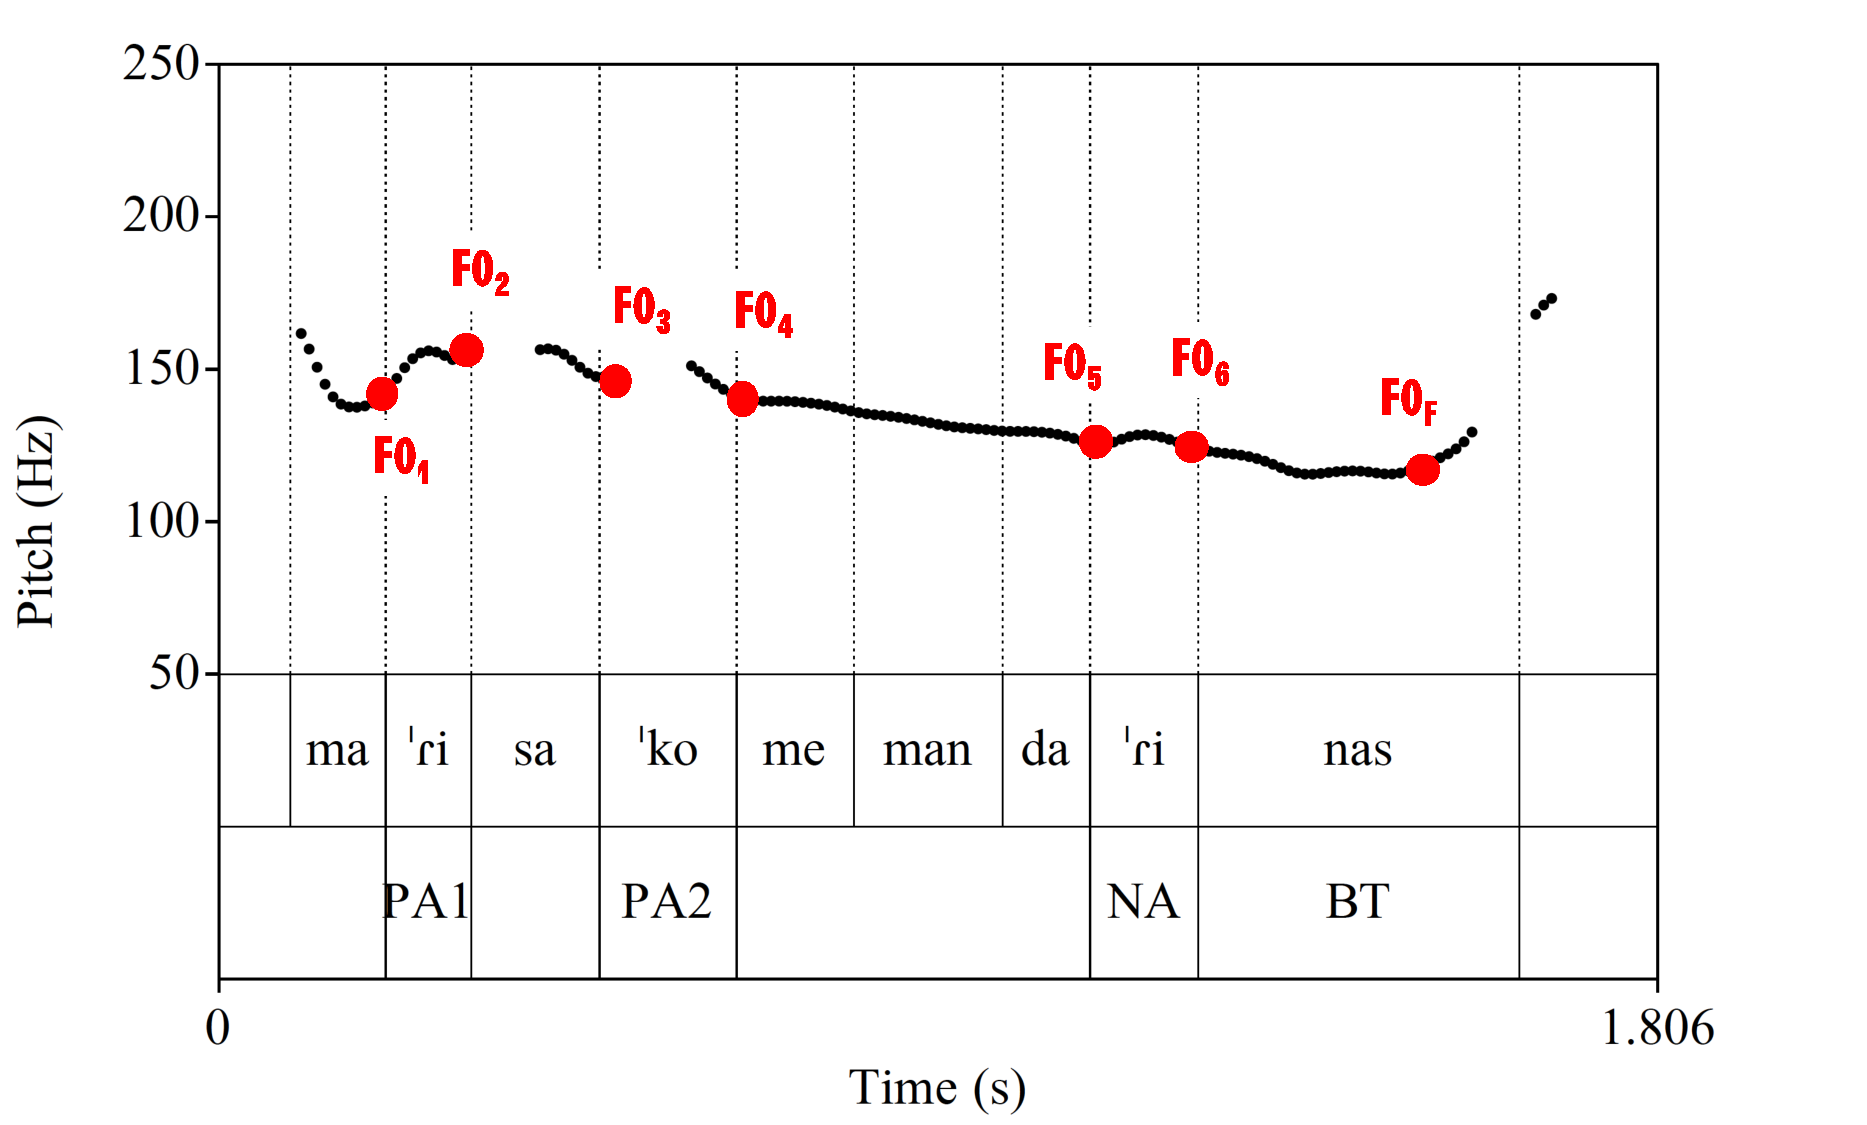
\includegraphics[width=\textwidth]{figures/a03HabilMethodology-img008.pdf}
\caption{Example of the F0 points analysed. Spectrogram and F0 trace for the statement \textit{Marisa come mandarinas} ‘Marisa eats tangerines’ (L1 Czech participant; Cz\_02\_M).}
\label{fig:3.8}
\end{figure}



\begin{figure}[p]
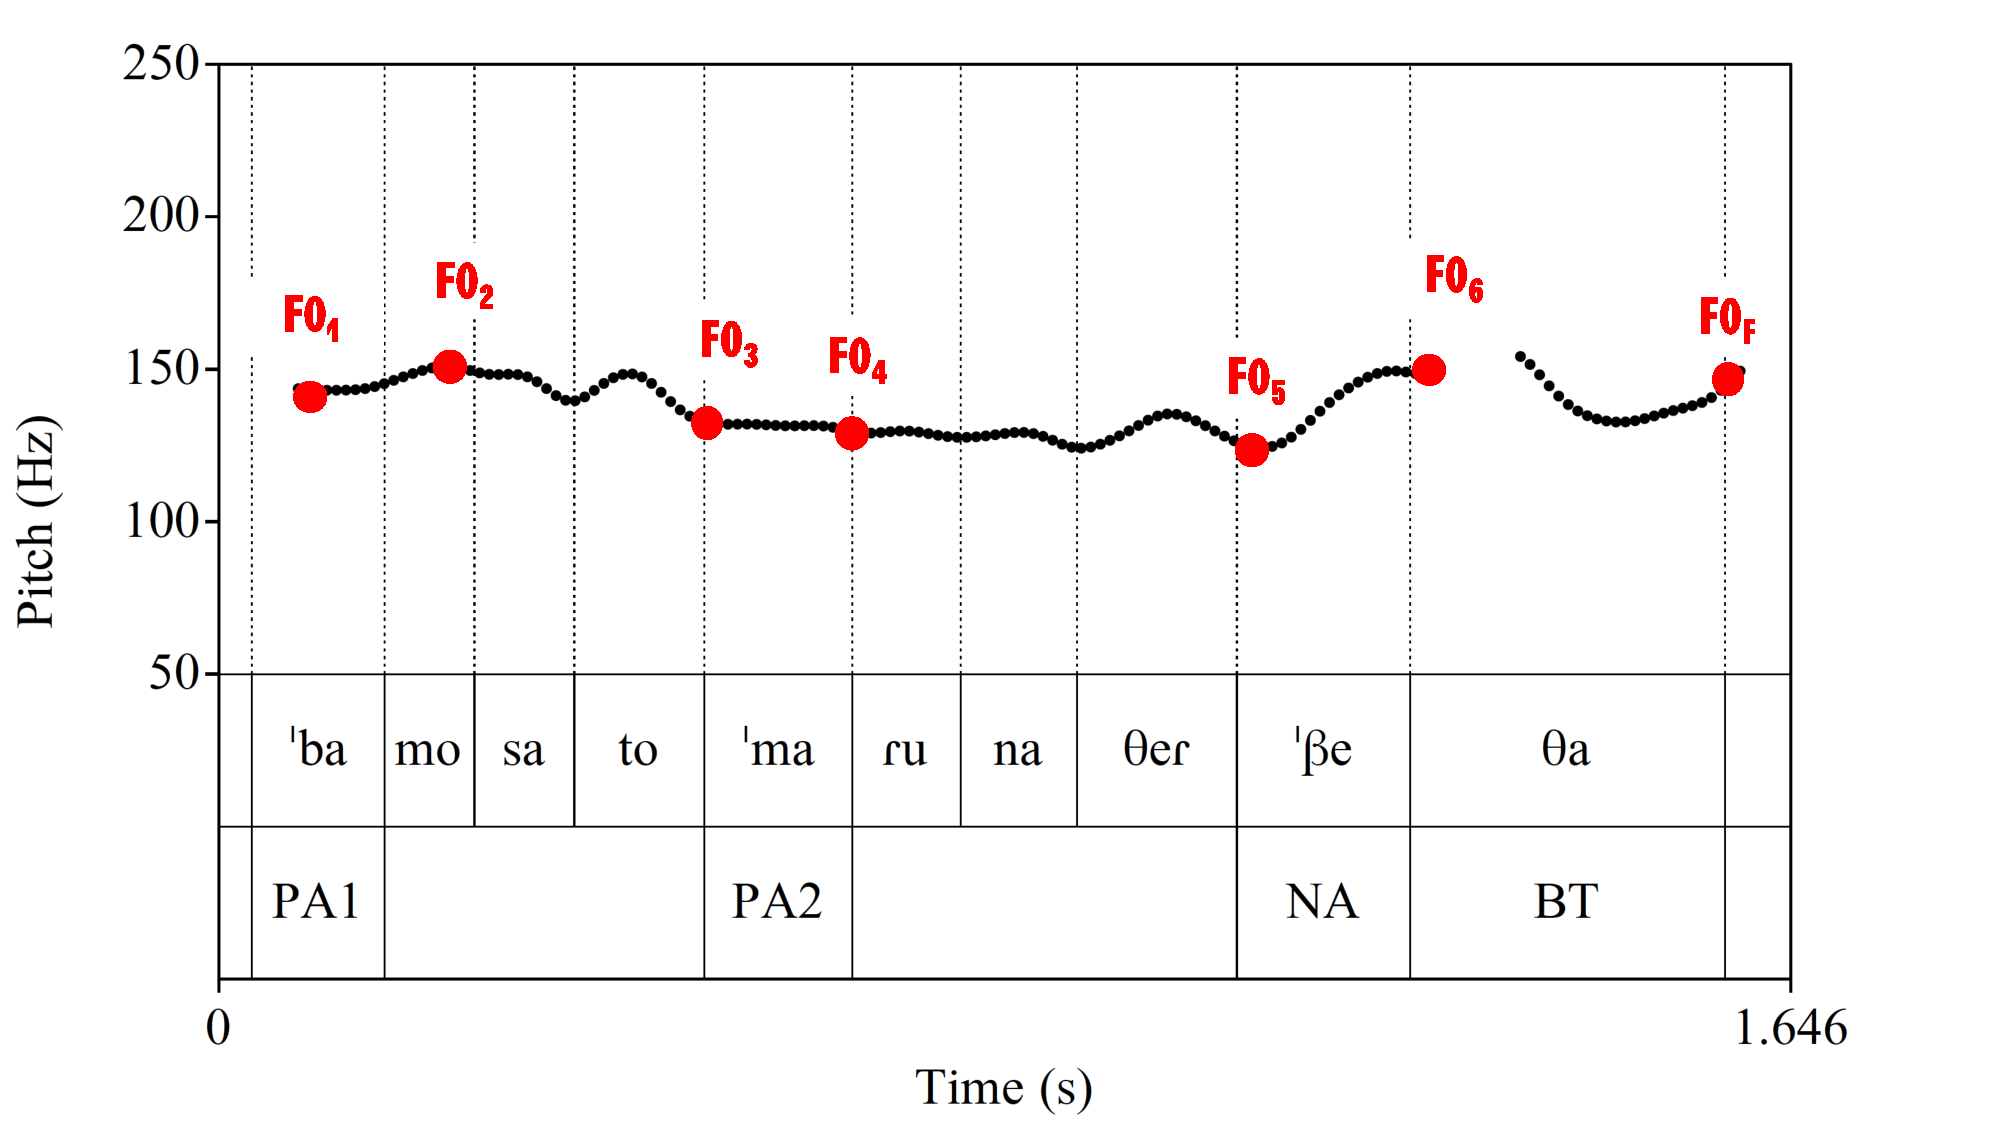
\includegraphics[width=\textwidth]{figures/a03HabilMethodology-img009.pdf}
\caption{Example of the F0 points analysed. Spectrogram and F0 trace for the yes/no question \textit{¿Vamos a tomar una cerveza?} ‘Shall we go have a beer?’ (L1 Czech participant; Cz\_02\_M).}
\label{fig:3.9}
\end{figure}


\begin{figure}[p]
%%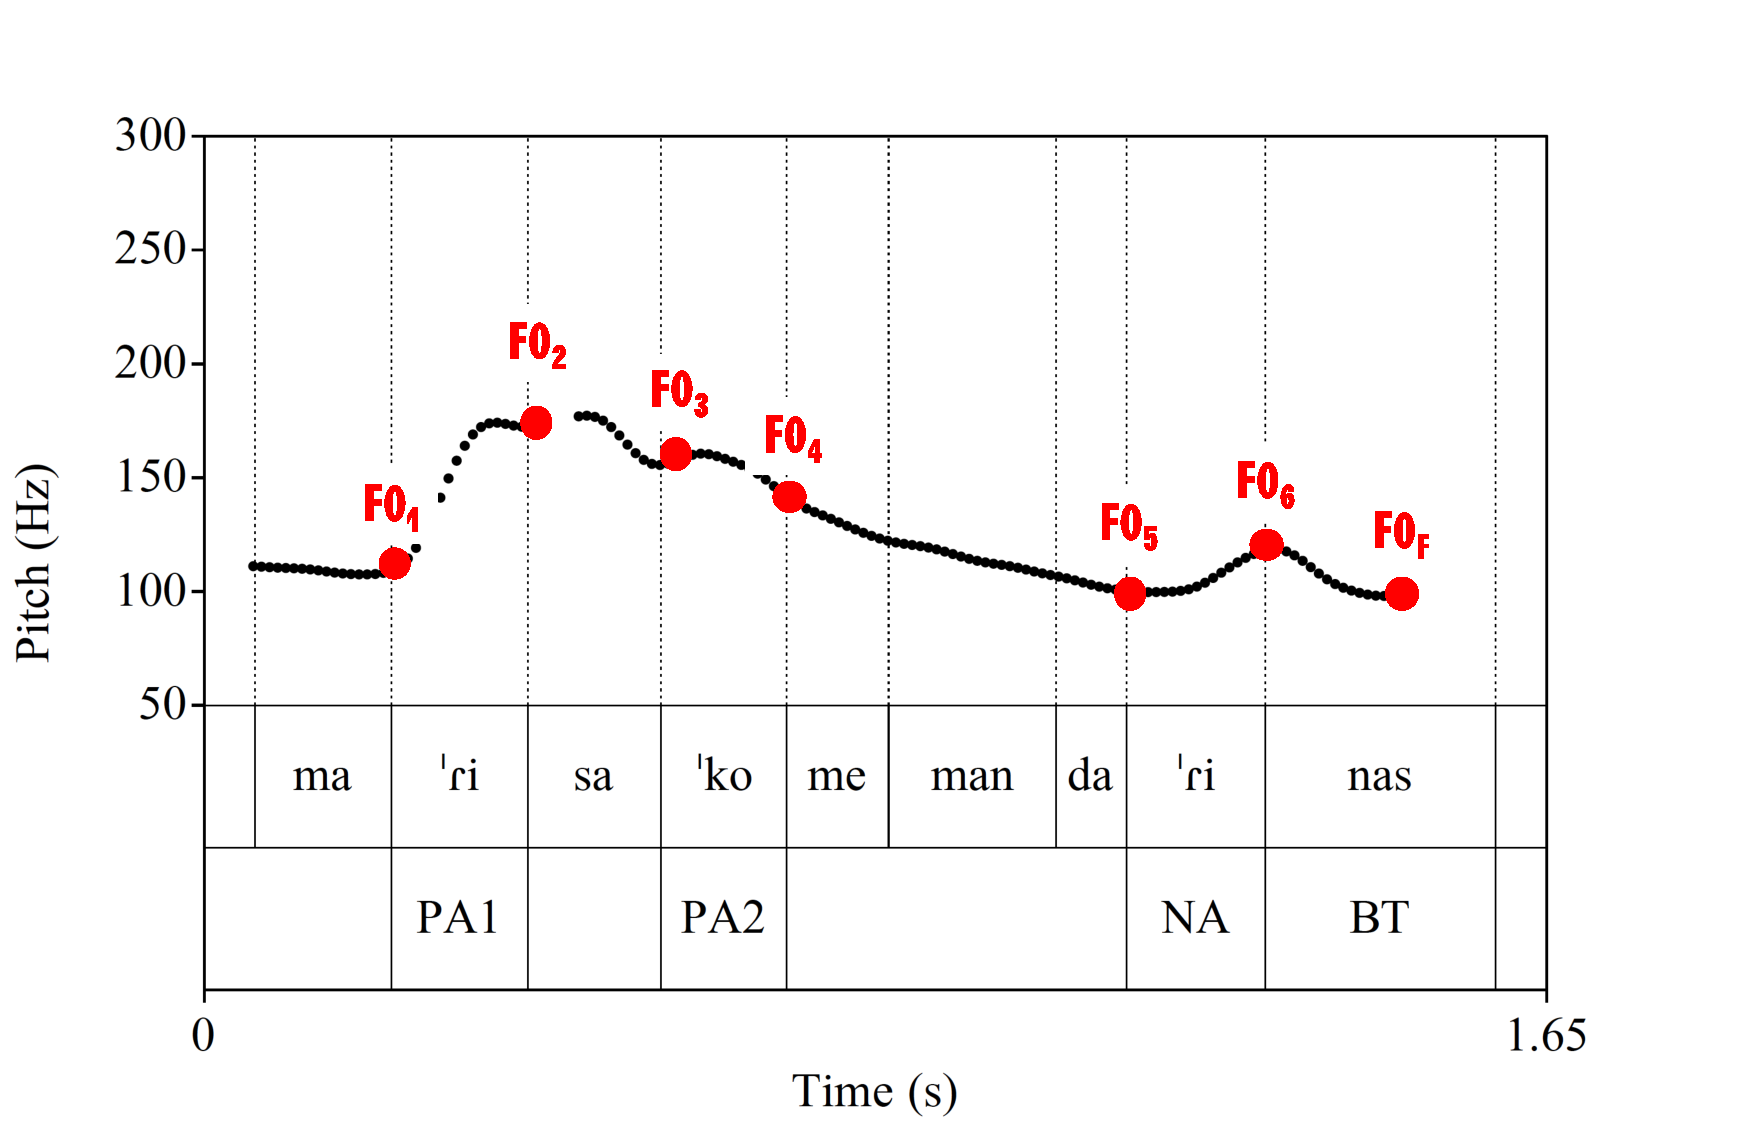
\includegraphics[width=\textwidth]{figures/a03HabilMethodology-img010.emf}
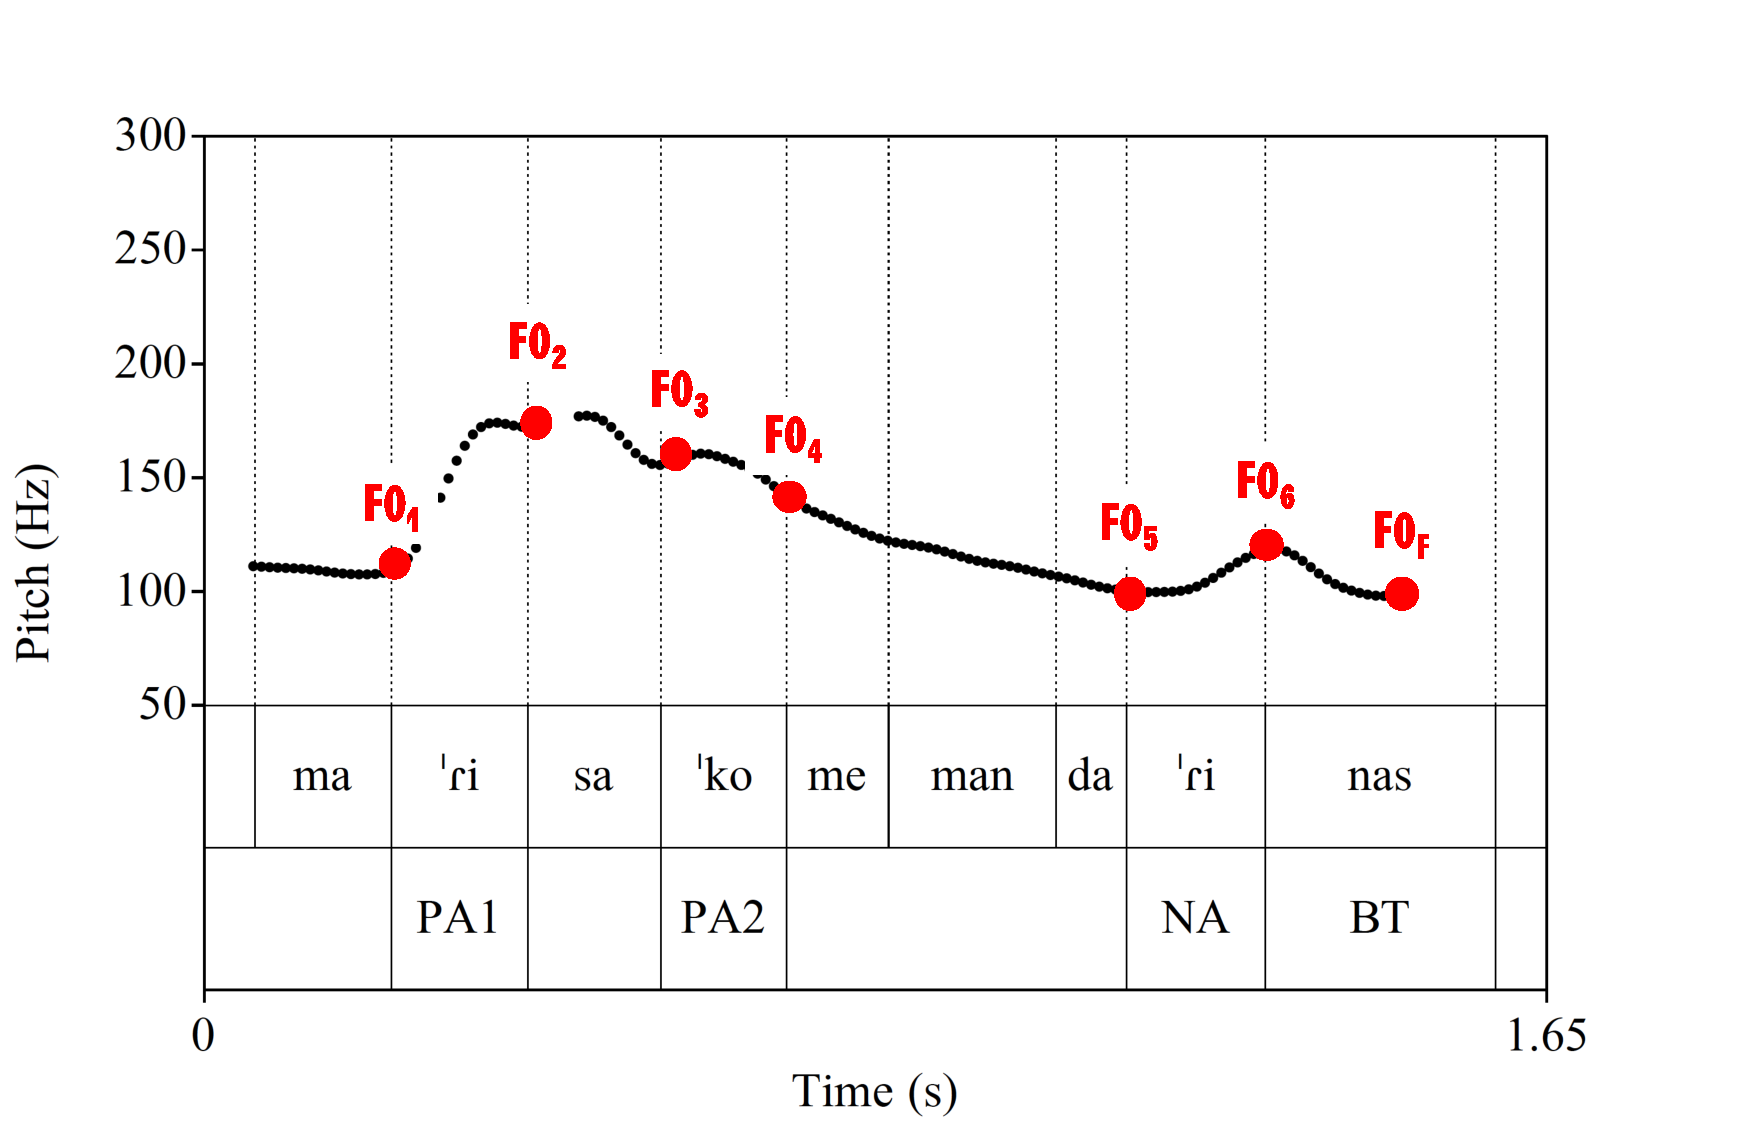
\includegraphics[width=\textwidth]{figures/a03HabilMethodology-img010.pdf}

\caption{Example of the F0 points analysed. Spectrogram and F0 trace for the statement \textit{Marisa come mandarinas} ‘Marisa eats tangerines’ (L1 German participant; Ge\_03\_M).}
\label{fig:3.10}
\end{figure}

\begin{figure}[p]
%%\includegraphics[width=\textwidth]{figures/a03HabilMethodology-img011.emf}
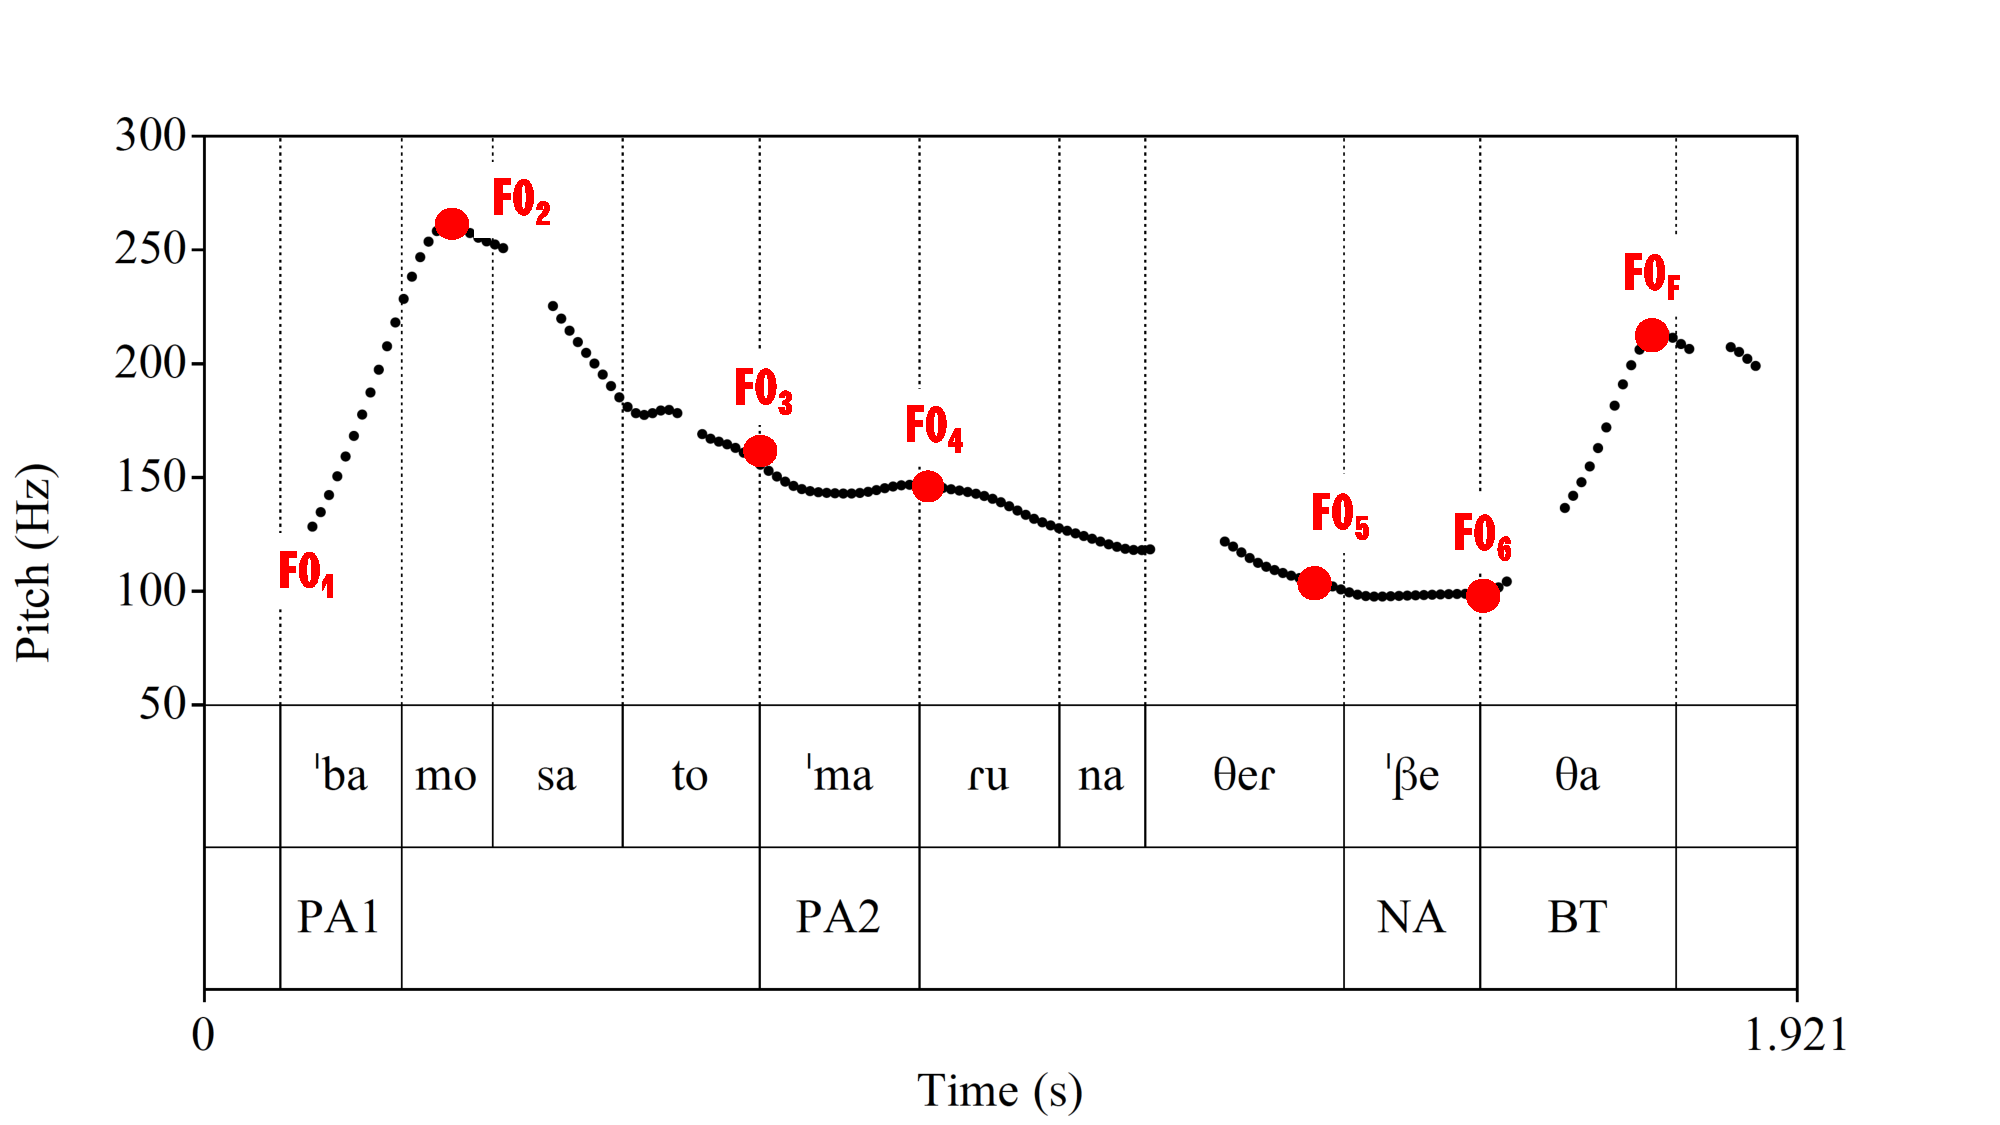
\includegraphics[width=\textwidth]{figures/a03HabilMethodology-img011.pdf}

\caption{Example of the F0 points analysed. Spectrogram and F0 trace for the yes/no question \textit{¿Vamos a tomar una cerveza?} ‘Shall we go have a beer?’ (L1 German participant; Ge\_03\_M).}
\label{fig:3.11}
\end{figure}


In a final step, I calculated a pitch change for each tonal event, by expressing ratios between F0 minimum vs. F0 maximum first. A pitch change refers here to a fixed ratio of frequencies if we understand a measurement as “the estimation of the ratio of some magnitude of a quantitative attribute to a unit of the same attribute” \citep[358]{Michell1997}. Magnitudes, such as maximal and minimal F0 within a tonal event, “stand in relations (\textit{ratios}) to one another and can be expressed as real numbers” \citep[356]{Michell1997}. The advantage of the ratio scale is that it has a non-arbitrary zero value. This is important because speech shows a range of variation and differences between speakers. For example, women have in general a wider F0-range in Hz than men. With ratios, the between-sex (or other speakers’ idiosyncratic) differences disappear. Let us imagine the two following scenarios: In speaker A, the min F0 point of the initial prenuclear accent has a value of 100\,Hz and the max F0 point 200\,Hz; in speaker B, the min. F0 point has a value of 300\,Hz and the max F0 point 400\,Hz. In both cases, the pitch change is 100\,Hz, but the ratios between the two F0 points are different, 1:2 in speaker A and 3:4 in speaker B, respectively. This means that the F0 max point has 50\% of the pitch change (increase) in speaker A, but only 25\% in speaker B; this was calculated as follows:

\begin{description}
\item [Speaker A:]   F0 max $-$ F0 min = 200\,Hz $-$ 100\,Hz / 200 * 100 = 50\%
\item [Speaker B:]   F0 max $-$ F0 min = 400\,Hz $-$ 300\,Hz / 400 * 100 = 25\%
\end{description}


And finally, I measured and compared the duration of the whole sentences. It is well known that speech rate can be a secondary prosodic characteristic of different types of sentences (see, e.g., \citealt{vanHeuvenvanZanten2005} regarding the speech rate of polarity questions in different languages). Since some disparities between the languages under study were observed, it was presumed that the learner groups might also differ from natives with respect to durational cues in L2 Spanish or Italian.
